\documentclass[tikz,crop,convert={density=200,outext=.png},border=0.4cm]{standalone}

\usepackage{pgfplots}
\usepackage{amsmath}
\usetikzlibrary{arrows.meta}
\usepackage{physics}
\usepackage{xcolor}
% STABLE NODE r
\definecolor{r_1}{RGB}{0,68,27}
\definecolor{r_2}{RGB}{0,109,44}
\definecolor{stab_r_3}{RGB}{102,194,164}
% STABLE NODE THETA
\definecolor{stab_theta_1}{RGB}{0,68,27}
\definecolor{stab_theta_2}{RGB}{0,109,44}
\definecolor{stab_theta_3}{RGB}{102,194,164}
% \definecolor{stab_theta_1}{RGB}{103,0,31}
%\definecolor{stab_theta_2}{RGB}{206,18,86}
%\definecolor{stab_theta_3}{RGB}{223,101,176}
% SADDLE POINT r
\definecolor{saddle_r_1}{RGB}{2,56,88}
\definecolor{saddle_r_2}{RGB}{5,112,176}
\definecolor{saddle_r_3}{RGB}{116,169,207}
% SADDLE POINT THETA
\definecolor{theta_1}{RGB}{2,56,88}
\definecolor{theta_2}{RGB}{5,112,176}
\definecolor{saddle_theta_3}{RGB}{116,169,207}
% \definecolor{saddle_theta_1}{RGB}{102,37,6}
%\definecolor{saddle_theta_2}{RGB}{204,76,2}
%\definecolor{saddle_theta_3}{RGB}{254,153,41}
\pgfplotsset{compat=newest,
    %width=6cm,
    %height=3cm,
    scale only axis=true,
    max space between ticks=25pt,
    try min ticks=5,
    every axis/.style={
        axis y line=middle,
        axis x line=middle,
        axis line style={thick,->,>=latex, shorten >=-.3cm}
    },
    every axis plot/.append style={thick},
    tick style={black, thick},
}
\tikzset{
    semithick/.style={line width=0.8pt},
}
\usepgfplotslibrary{groupplots}
\usepgfplotslibrary{dateplot}
% Document begins
\begin{document}

% =========================================================================================================
% r trans figure stable node
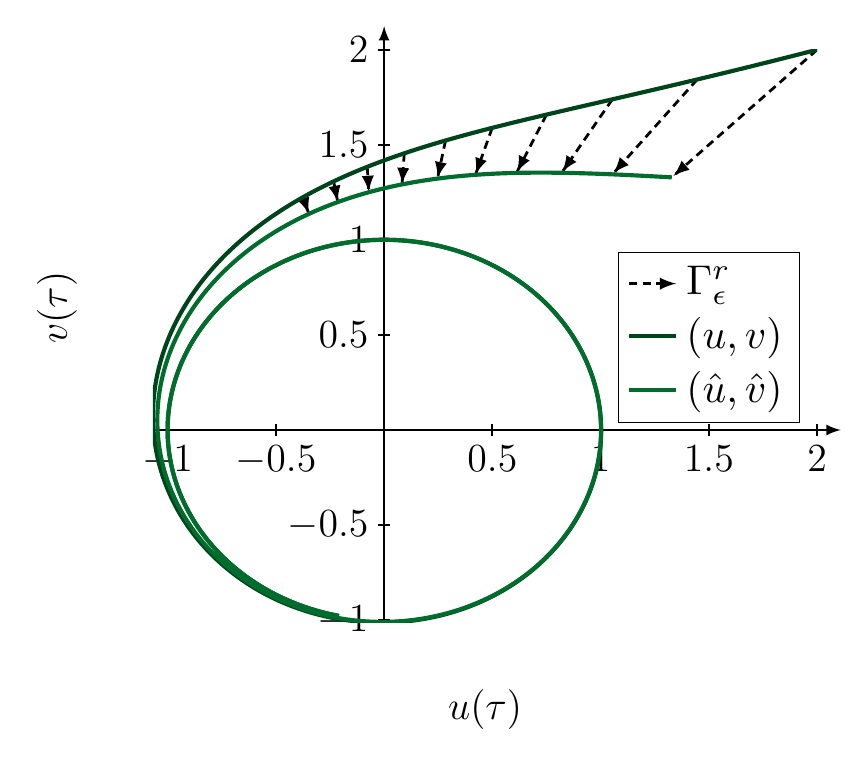
\begin{tikzpicture}
  % The axis of the plot
\begin{axis}[
    xlabel={$u(\tau)$},
    ylabel={$v(\tau)$},
    x label style={at={(axis description cs:0.5,-0.1)},anchor=north},
    y label style={at={(axis description cs:-0.1,0.55)},rotate=90,anchor=south},
    scaled x ticks = false,
    xtick={-1,-0.5,...,2},
    % ymax = 4.5,
    %xmax = 4.5,
    legend style={at={(axis description cs:0.7,0.4975)},anchor=west,nodes={scale=1.5, transform shape}},
    label style={font=\Large},
    tick label style={font=\Large},
    legend cell align={left},
    grid style=dashed,
]
\addplot[
color=black,->,>=latex,densely dashed,line width=1.0pt
]
coordinates {%
(2.0,2.0)
(1.9762301738739774,1.9762301738739774)
(1.9531696031918422,1.9531696031918422)
(1.930787504013317,1.930787504013317)
(1.909054832637882,1.909054832637882)
(1.8879441803872223,1.8879441803872223)
(1.867429679733759,1.867429679733759)
(1.8474868489398704,1.8474868489398704)
(1.828092536134045,1.828092536134045)
(1.8092248163393556,1.8092248163393556)
(1.7908629363895936,1.7908629363895936)
(1.7729872260245825,1.7729872260245825)
(1.7555789752038424,1.7555789752038424)
(1.738620447714456,1.738620447714456)
(1.7220947983770554,1.7220947983770554)
(1.705986010568205,1.705986010568205)
(1.6902788438505063,1.6902788438505063)
(1.6749587953951932,1.6749587953951932)
(1.6600120471560196,1.6600120471560196)
(1.645425435386674,1.645425435386674)
(1.631186403683989,1.631186403683989)
(1.6172829774767739,1.6172829774767739)
(1.6037037183056597,1.6037037183056597)
(1.5904377006016652,1.5904377006016652)
(1.5774744900021935,1.5774744900021935)
(1.564804117747995,1.564804117747995)
(1.552417033444617,1.552417033444617)
(1.5403041022386164,1.5403041022386164)
(1.5284565801124648,1.5284565801124648)
(1.5168660852724338,1.5168660852724338)
(1.5055245887466915,1.5055245887466915)
(1.4944243906978512,1.4944243906978512)
(1.4835581054483655,1.4835581054483655)
(1.4729186463243327,1.4729186463243327)
(1.462499208252797,1.462499208252797)
(1.452293256537062,1.452293256537062)
(1.4422945119709352,1.4422945119709352)
(1.4324969386622937,1.4324969386622937)
(1.422894733179857,1.422894733179857)
(1.4134823110921915,1.4134823110921915)
(1.4042542999955943,1.4042542999955943)
(1.3952055301213724,1.3952055301213724)
(1.386331022194954,1.386331022194954)
(1.3776259749599313,1.3776259749599313)
(1.3690857650995163,1.3690857650995163)
(1.3607059373666506,1.3607059373666506)
(1.3524821927045978,1.3524821927045978)
(1.3444103831546461,1.3444103831546461)
(1.3364865083624704,1.3364865083624704)
};
\addlegendentry{$\Gamma_{\epsilon}^{r}$}
\addplot[
forget plot,
color=black,->,>=latex,densely dashed,line width=1.0pt
]
coordinates {%
(1.446101254320559,1.8435702685464732)
(1.4334367558672543,1.827424861891989)
(1.42107337446791,1.8116633359971506)
(1.409000651852031,1.7962723580773505)
(1.3972087560912985,1.7812393938438051)
(1.3856882423995898,1.7665524025581252)
(1.3744300919450045,1.7521998865120425)
(1.3634256866009964,1.7381708588387492)
(1.3526667763796363,1.724454801995012)
(1.3421454604315302,1.7110416435388114)
(1.3318541764282674,1.6979217425934954)
(1.3217856773880075,1.6850858603037504)
(1.3119330153660558,1.672525139043439)
(1.302289540725293,1.6602311014855051)
(1.2928488711445707,1.648195611092152)
(1.2836048681119483,1.636410842147115)
(1.274551630723676,1.624869271850259)
(1.2656835167340144,1.6135637071530604)
(1.256995089971163,1.6024872177215082)
(1.248481128686264,1.5916331465798783)
(1.2401366108438014,1.5809950913581177)
(1.2319567027453473,1.5705668897887621)
(1.2239367561433876,1.5603426160274825)
(1.2160722923066845,1.5503165603387214)
(1.208359000220887,1.5404832268017332)
(1.2007927261200848,1.5308373199648253)
(1.1933694657912053,1.5213737350345757)
(1.1860853614596256,1.5120875539054404)
(1.1789366896164934,1.5029740296413416)
(1.1719198569291462,1.4940285812620464)
(1.1650313977642834,1.4852467905855669)
(1.1582679677950953,1.4766243940781731)
(1.1516263408017586,1.468157278775487)
(1.1451033962008166,1.4598414663842427)
(1.1386961168065572,1.4516731104283682)
(1.1324015901324258,1.4436484979080966)
(1.1262170006722936,1.4357640394596995)
(1.1201396228046492,1.4280162603093554)
(1.114166821716964,1.4204018014515816)
(1.1082960484859208,1.4129174133772384)
(1.1025248351888277,1.4055599498412845)
(1.0968507929361797,1.398326365354579)
(1.0912716089239585,1.3912137114259897)
(1.0857850426270461,1.3842191317095447)
(1.0803889230298231,1.3773398584738434)
(1.0750811466757793,1.3705732101155947)
(1.0698596747055829,1.363916587383582)
(1.0647225298084901,1.357367469492148)
(1.0596677947622486,1.350923412259787)
};
\addplot[
forget plot,
color=black,->,>=latex,densely dashed,line width=1.0pt
]
coordinates {%
(1.0541264523851241,1.739099558958013)
(1.0470073093726764,1.7273543850795923)
(1.0400296520818413,1.7158426345779378)
(1.033189325968556,1.704557453279407)
(1.026482514810077,1.6934925451734255)
(1.0199054853214942,1.6826417510803944)
(1.0134546435060392,1.6719991416185205)
(1.007126529565168,1.6615590088064616)
(1.0009178064795974,1.6513158472243032)
(0.9948252668068434,1.6412643652281476)
(0.9888458038814754,1.6313994374362453)
(0.9829764248855392,1.6217161262926019)
(0.9772142426487292,1.6122096685388874)
(0.9715564684717037,1.6028754633743307)
(0.966000408122125,1.593709065849979)
(0.9605434614542027,1.5847061862410214)
(0.9551831197977241,1.5758626857392048)
(0.9499169567268386,1.5671745612231607)
(0.944742622355347,1.5586379358467635)
(0.9396578380496706,1.550249050316579)
(0.9346604067165738,1.5420042798645643)
(0.9297482070252725,1.5339001247156956)
(0.924919179654108,1.5259331873977047)
(0.9201713323839763,1.5181001811442298)
(0.9155027374007454,1.5103979254443376)
(0.9109115250886498,1.502823335802856)
(0.9063958846801843,1.4953734248125699)
(0.9019540624247685,1.48804529913288)
(0.8975843566344376,1.4808361513161776)
(0.8932851177383687,1.4737432598977989)
(0.8890547470764711,1.4667639874056908)
(0.8848916925186759,1.4598957731331068)
(0.8807944483127936,1.4531361328876025)
(0.8767615543455549,1.446482657771899)
(0.8727915919061722,1.4399330071946)
(0.8688831830057405,1.4334849077473384)
(0.8650349893288649,1.4271361514751693)
(0.8612457119157749,1.4208845953521219)
(0.857514088848411,1.4147281574637012)
(0.8538388948484938,1.4086648163437823)
(0.8502189395714252,1.4026926081598843)
(0.8466530619985839,1.396809617461572)
(0.8431401349599512,1.3910139846418903)
(0.8396790629860117,1.3853039023934268)
(0.8362687808891581,1.3796776133679105)
(0.8329082508082517,1.3741334053003245)
(0.8295964632355808,1.3686696127031814)
(0.8263324360120405,1.3632846152087708)
(0.8231152132176289,1.3579768357386977)
};
\addplot[
forget plot,
color=black,->,>=latex,densely dashed,line width=1.0pt
]
coordinates {%
(0.7500731096845435,1.6587429197626766)
(0.7460465741728154,1.6498384714028878)
(0.7420891566058292,1.6410868733452753)
(0.7381990945041578,1.6324842279694154)
(0.7343747932714887,1.6240270089185989)
(0.7306146826680706,1.6157117436992292)
(0.7269172396096895,1.6075350640994301)
(0.7232809875517857,1.599493704827056)
(0.7197044974919439,1.5915845057266385)
(0.7161863833022961,1.5838044014572705)
(0.7127253050098258,1.5761504287468049)
(0.7093199607761411,1.5686197086555933)
(0.7059690863626638,1.5612094453937797)
(0.7026714559919685,1.5539169282261056)
(0.6994258813901073,1.546739529354064)
(0.6962312078783248,1.5396746952729552)
(0.6930863157402153,1.532719949795277)
(0.6899901156602042,1.5258728839631919)
(0.6869415524018495,1.5191311641828744)
(0.6839396017387608,1.51249252543742)
(0.6809832679686197,1.5059547657892451)
(0.6780715820438167,1.4995157422460987)
(0.6752036003284871,1.4931733680123225)
(0.6723784032206283,1.4869256094417402)
(0.6695951029297847,1.4807705032375573)
(0.6668528349880471,1.4747061376794286)
(0.664150756482751,1.4687306487151757)
(0.6614880472272088,1.462842222549792)
(0.6588639108172913,1.4570390979820111)
(0.6562775710167232,1.4513195584105993)
(0.6537282716859564,1.4456819316770617)
(0.6512152771611952,1.4401245909038363)
(0.6487378714709616,1.4346459527617716)
(0.6462953565483943,1.4292444735167322)
(0.6438870521305913,1.4239186488069995)
(0.6415122961233568,1.418667014449889)
(0.6391704433013148,1.4134881435671265)
(0.6368608642163052,1.4083806441708304)
(0.6345829453451568,1.4033431594903036)
(0.6323360893181083,1.3983743684771708)
(0.6301197129707617,1.3934729814973914)
(0.6279332473388874,1.3886377403197665)
(0.6257761372434653,1.3838674171982845)
(0.6236478410977764,1.3791608144455152)
(0.6215478309157826,1.3745167644511396)
(0.6194755913641824,1.3699341275856285)
(0.6174306197578722,1.3654117921902036)
(0.6154124258722439,1.360948674161746)
(0.613420530719644,1.3565437142470063)
};
\addplot[
forget plot,
color=black,->,>=latex,densely dashed,line width=1.0pt
]
coordinates {%
(0.4992809294283036,1.5890358689295765)
(0.49710426114785045,1.582108298160227)
(0.4949606411561439,1.5752859084885915)
(0.4928493508846686,1.5685664129634211)
(0.49076969690401595,1.561947604642416)
(0.48872103018249224,1.5554274178856116)
(0.4867027064693602,1.5490038022691486)
(0.4847140972951044,1.5426747575952549)
(0.48275459499505224,1.536438349880668)
(0.48082360617941405,1.530292690574064)
(0.4789205548052037,1.5242359463329036)
(0.4770448782782707,1.5182663266175689)
(0.475196033246431,1.5123821021288637)
(0.47337348581630984,1.5065815736716601)
(0.4715767178531809,1.5008630922050745)
(0.46980522419642523,1.4952250499802506)
(0.46805851341924315,1.4896658829582572)
(0.46633610588507746,1.484184064624363)
(0.4646375349189607,1.478778109716026)
(0.4629623450302584,1.4734465685665088)
(0.46131009192381534,1.4681880271403531)
(0.45968034355205695,1.4630011103818479)
(0.4580726788073115,1.4578844780531524)
(0.456486686859789,1.4528368226273132)
(0.45492196636928933,1.4478568667794098)
(0.45337812532162086,1.4429433628659318)
(0.4518547803336087,1.4380950907128631)
(0.4503515566751071,1.433310857685742)
(0.448868092102316,1.4285895108897597)
(0.44740403174877563,1.4239299209095913)
(0.4459590284320167,1.4193309827853546)
(0.44453274288152633,1.4147916167381467)
(0.4431248444766417,1.4103107705185003)
(0.44173501031313267,1.4058874164356427)
(0.44036292455808934,1.401520549304331)
(0.43900827847477886,1.397209186523962)
(0.4376707705838785,1.3929523685917196)
(0.43635010659667534,1.3887491588899743)
(0.4350459985020847,1.384598640780583)
(0.43375816463493416,1.3804999178222122)
(0.4324863296423799,1.3764521136634542)
(0.4312302246572056,1.3724543725943759)
(0.4299895865778109,1.3685058572549746)
(0.4287641578920344,1.3646057480744704)
(0.42755368664894144,1.3607532431815135)
(0.4263579268114109,1.3569475595263474)
(0.42517663747182965,1.3531879303846372)
(0.4240095827491378,1.3494736050298026)
(0.42285653173647475,1.3458038485663921)
};
\addplot[
forget plot,
color=black,->,>=latex,densely dashed,line width=1.0pt
]
coordinates {%
(0.283677298722318,1.5226291721826193)
(0.28265680846548485,1.5171517221294046)
(0.2816502745811209,1.5117491824759832)
(0.28065744751694,1.5064202137581375)
(0.2796780469098205,1.5011633111354385)
(0.27871183451118087,1.4959771958159558)
(0.27775856591929293,1.4908605559809338)
(0.2768180033768367,1.4858121154752733)
(0.2758899136137187,1.480830622228925)
(0.2749740704460553,1.4759148622068532)
(0.2740702523476307,1.4710636463739113)
(0.2731782437290531,1.4662758175606718)
(0.2722978330301416,1.4615502402243743)
(0.2714288148858227,1.4568858120743051)
(0.2705709891127559,1.4522814586325439)
(0.2697241582035231,1.447736119784101)
(0.2688881304352909,1.4432487664625684)
(0.268062718101897,1.4388183911608947)
(0.2672477379322048,1.4344440101768936)
(0.2664430109972585,1.4301246631149005)
(0.2656483619242072,1.4258594086665346)
(0.2648636198022894,1.4216473294735423)
(0.26408861696811525,1.4174875256078374)
(0.26332318968774426,1.413379118232533)
(0.262567178171448,1.4093212496811776)
(0.2618204262056835,1.4053130814823867)
(0.26108278098579446,1.401353793461869)
(0.2603540928286009,1.3974425821997616)
(0.2596342151428862,1.39357866087222)
(0.25892300426736264,1.3897612583817032)
(0.25822031928422157,1.3859896183562084)
(0.25752602209652786,1.3822629995646862)
(0.25683997907559175,1.378580684759256)
(0.2561620588188667,1.3749419686407927)
(0.25549213236617285,1.3713461590194984)
(0.25483007335476116,1.367792577647206)
(0.25417575802021575,1.3642805602222214)
(0.2535290655436371,1.3608094582528192)
(0.2528898773709725,1.35737863540377)
(0.25225807728180405,1.3539874678655555)
(0.2516335513564635,1.3506353441778622)
(0.251016187985009,1.3473216652777618)
(0.25040587803322567,1.3440458453907138)
(0.24980251438918372,1.3408073095967306)
(0.24920599201866706,1.3376054941278892)
(0.24861620791620048,1.3344398461054714)
(0.24803306115052912,1.331309823784072)
(0.24745645289521429,1.3282148967158223)
(0.24688628617790798,1.325154544404628)
};
\addplot[
forget plot,
color=black,->,>=latex,densely dashed,line width=1.0pt
]
coordinates {%
(0.09319363131665603,1.4551819451667813)
(0.09291359564167742,1.4508092981041636)
(0.09263706473450943,1.4464913766141838)
(0.09236398201154905,1.4422272971661076)
(0.09209428228949439,1.4380160419482815)
(0.09182791094276388,1.4338567580037065)
(0.09156481343470234,1.4297485937639351)
(0.09130493512091907,1.4256906959782716)
(0.09104822301623326,1.4216822373039308)
(0.09079462481529352,1.4177224010133975)
(0.09054408975068004,1.4138103943933533)
(0.09029656796108938,1.409945438879131)
(0.09005201072256735,1.4061267736653258)
(0.08981037037722481,1.402353654592719)
(0.08957160002066211,1.3986253492675358)
(0.08933565426314279,1.39494114894687)
(0.08910248839715156,1.3913003555404329)
(0.08887205834604844,1.3877022808088049)
(0.08864432123619649,1.3841462552969865)
(0.08841923498492048,1.3806316219005348)
(0.08819675835878431,1.3771577367755423)
(0.08797685108481587,1.373723971075369)
(0.08775947351234062,1.3703297056703077)
(0.08754458693607658,1.3669743361925841)
(0.08733215341982344,1.3636572702833318)
(0.08712213563795805,1.3603779251176085)
(0.08691449709958106,1.3571357309043541)
(0.08670920209702704,1.3539301300824)
(0.08650621563965293,1.3507605762865988)
(0.0863055034256891,1.3476265339082931)
(0.08610703179906756,1.3445274774212008)
(0.08591076770996567,1.3414628907653245)
(0.08571667872147488,1.338432267451079)
(0.0855247329651471,1.335435109865165)
(0.08533489911169465,1.3324709288130627)
(0.08514714636846428,1.3295392434795874)
(0.08496144490366173,1.3266395880529893)
(0.08477776536841317,1.3237715042621332)
(0.08459607884823157,1.3209345406186617)
(0.08441635695236542,1.3181282538121424)
(0.08423857179701609,1.3153522084480127)
(0.08406269603470395,1.3126059775061207)
(0.08388870290864477,1.309889143189791)
(0.08371656608418421,1.3072012942937412)
(0.08354625969476503,1.3045420269218406)
(0.08337775833193137,1.3019109443310315)
(0.08321103703378509,1.29930765675108)
(0.0830460713423208,1.2967317822798392)
(0.0828828372325421,1.294182945776428)
};
\addplot[
forget plot,
color=black,->,>=latex,densely dashed,line width=1.0pt
]
coordinates {%
(-0.07798193781933803,1.3840144606983118)
(-0.07778431853379573,1.3805071363543455)
(-0.07758898881104818,1.3770404469074498)
(-0.0773959162304643,1.3736138169599932)
(-0.07720506211862567,1.3702265601405956)
(-0.07701639144195495,1.3668780546773567)
(-0.07682987282129101,1.363567743656535)
(-0.07664547367539408,1.3602950488300352)
(-0.07646316185468324,1.3570593996107947)
(-0.07628290616732558,1.3538602424097501)
(-0.07610467565496339,1.3506970277815318)
(-0.0759284403255505,1.3475692234307544)
(-0.07575417059370596,1.3444763042794807)
(-0.07558183745125097,1.3414177554938906)
(-0.07541141261198175,1.338393075053694)
(-0.07524286804206776,1.3354017654176915)
(-0.07507617643236143,1.332443341906274)
(-0.07491131120481075,1.3295173328152317)
(-0.07474824599810646,1.3266232702870815)
(-0.07458695485804812,1.323760693689659)
(-0.07442741248346942,1.3209291539807766)
(-0.07426959401738069,1.3181282100014406)
(-0.07411347499952728,1.315357427633866)
(-0.07395903149920725,1.3126163821587076)
(-0.0738062400404664,1.309904656927431)
(-0.07365507744900009,1.3072218406451441)
(-0.07350552109486513,1.3045675316782188)
(-0.07335754874489149,1.3019413354349108)
(-0.07321113845967418,1.2993428625371846)
(-0.07306626876214502,1.296771731812505)
(-0.07292291859686423,1.2942275695713492)
(-0.07278106729235823,1.2917100089387825)
(-0.0726406945475564,1.2892186896137394)
(-0.07250178041771976,1.2867532576192866)
(-0.07236430528352622,1.2843133647539529)
(-0.07222824985286078,1.2818986686235008)
(-0.07209359515166586,1.2795088324785395)
(-0.0719603225043407,1.2771435248666552)
(-0.07182841351982013,1.2748024193853391)
(-0.07169785007765336,1.2724851944349156)
(-0.07156861452653632,1.2701915367420702)
(-0.07144068962777972,1.2679211403565294)
(-0.07131405828729974,1.2656737018944597)
(-0.07118870369259558,1.2634489229695316)
(-0.07106460930471772,1.2612465100503711)
(-0.07094175885023436,1.2590661743179836)
(-0.0708201363456624,1.2569076320993493)
(-0.07069972612952946,1.254770605436459)
(-0.07058051275258133,1.2526548201377257)
};
\addplot[
forget plot,
color=black,->,>=latex,densely dashed,line width=1.0pt
]
coordinates {%
(-0.23322791946942856,1.3074599868720134)
(-0.2327256193699895,1.3046441263913628)
(-0.23222876103192006,1.3018587720579393)
(-0.2317372751457864,1.2991035353277314)
(-0.23125108083224907,1.2963779627966174)
(-0.23077009396160203,1.2936815828391388)
(-0.2302942474087855,1.2910140191567379)
(-0.22982347053556998,1.2883748757562639)
(-0.22935769262889547,1.2857637562250717)
(-0.2288968443150444,1.2831802716587792)
(-0.22844085793102875,1.2806240427432396)
(-0.22798966593749032,1.2780946908573654)
(-0.2275432034045508,1.275591852008638)
(-0.22710140569843765,1.2731151638644875)
(-0.2266642094544918,1.2706642712069092)
(-0.22623155267690356,1.2682388264915745)
(-0.22580337445874576,1.265838488278358)
(-0.22537961429741613,1.2634629173937513)
(-0.22496021353880108,1.2611117850267501)
(-0.22454511483616593,1.2587847696954269)
(-0.22413426103803127,1.256481551012443)
(-0.2237275958613425,1.25420181345879)
(-0.22332506437106406,1.2519452490723637)
(-0.2229266125892308,1.249711555256332)
(-0.22253218720420104,1.247500433149227)
(-0.22214173595592834,1.2453115897847526)
(-0.22175520755487457,1.2431447376372178)
(-0.22137255150049728,1.2409995936039873)
(-0.22099371791620231,1.238875878080238)
(-0.22061865804498632,1.2367733177374975)
(-0.22024732390399537,1.234691643587123)
(-0.21987966803488804,1.232630589580853)
(-0.2195156438843267,1.2305898947438163)
(-0.21915520577010503,1.2285693029846456)
(-0.2187983087742115,1.2265685624959977)
(-0.21844490871839561,1.2245874256175797)
(-0.21809496213973412,1.2226256486991751)
(-0.21774842626161042,1.2206829919379565)
(-0.2174052589298075,1.2187592190202257)
(-0.21706541864151133,1.2168540972840067)
(-0.21672886451196682,1.2149673975321202)
(-0.21639555624201703,1.21309889385021)
(-0.21606545409307784,1.211248363466454)
(-0.2157385188621128,1.2094155866112728)
(-0.21541471198086837,1.2076003470736394)
(-0.21509399616079164,1.2058024358164405)
(-0.21477633433660495,1.2040216450542296)
(-0.21446168990794096,1.2022577696078154)
(-0.21415002682197548,1.2005106073674974)
};
\addplot[
forget plot,
color=black,->,>=latex,densely dashed,line width=1.0pt
]
coordinates {%
(-0.37445604602258903,1.2245267732124638)
(-0.37376636367463917,1.2222714097083962)
(-0.373083728918348,1.2200390928736633)
(-0.37240805594258874,1.21782954209316)
(-0.37173925623448445,1.2156424679166598)
(-0.3710772238140944,1.2134775237740476)
(-0.37042187165653245,1.2113344250810472)
(-0.3697731187812383,1.2092129070192228)
(-0.36913088030849484,1.2071126920193185)
(-0.36849507171008494,1.2050335036615358)
(-0.3678656107458605,1.2029750730084)
(-0.36724241678999936,1.2009371364015222)
(-0.3666254083783377,1.198919427441012)
(-0.36601450875352776,1.1969216951189652)
(-0.36540964001630805,1.1949436846932502)
(-0.3648107263048943,1.1929851480845879)
(-0.36421769288253725,1.1910458408927305)
(-0.36363046674953087,1.1891255243978194)
(-0.36304897526445856,1.1872239610516553)
(-0.3624731469538491,1.185340917125393)
(-0.3619029122850309,1.1834761652368906)
(-0.3613382031455077,1.181629482648189)
(-0.36077895149815575,1.1798006468678095)
(-0.36022509010805015,1.1779894380275813)
(-0.35967655337658155,1.176195641610329)
(-0.35913327681706786,1.174419046735044)
(-0.35859519670871576,1.1726594450252867)
(-0.35806225026648014,1.1709166311646542)
(-0.3575343758777914,1.169190403670911)
(-0.357011513110142,1.1674805649208004)
(-0.3564936016747176,1.1657869177609632)
(-0.3559805829072471,1.1641092703505374)
(-0.3554723988188647,1.1624474330573367)
(-0.35496899240896246,1.160801219480924)
(-0.354470307271195,1.1591704451641902)
(-0.35397628781891816,1.157554928330569)
(-0.3534868795392142,1.1559544907147394)
(-0.3530020287629459,1.1543689568106679)
(-0.3525216826402247,1.1527981537913854)
(-0.35204578911587886,1.1512419114287642)
(-0.3515742969049214,1.1497000620132958)
(-0.3511071554616686,1.1481724402531024)
(-0.3506443149090543,1.1466588830427844)
(-0.3501857260822735,1.1451592296061424)
(-0.3497313404900389,1.1436733213694792)
(-0.3492811102811251,1.1422010018521953)
(-0.34883498821929954,1.1407421165848088)
(-0.3483929276582533,1.1392965130269754)
(-0.3479548825165317,1.1378640404855085)
};
\addplot[
color=r_1,line width=1.5pt,
]
coordinates {%
(2.0,2.0)
(1.8909237144620223,1.9682726491844558)
(1.7896932832135488,1.93922916589428)
(1.6953480903861957,1.9125154277625709)
(1.6070772150424197,1.8878318291790523)
(1.5241913742499995,1.8649230698181607)
(1.446101254320559,1.8435702685464732)
(1.3723000282364406,1.8235846012500532)
(1.302349524824366,1.8048022682108587)
(1.2358691344755055,1.787080457614985)
(1.1725266962242977,1.7702940304257995)
(1.1120311492122734,1.75433284760152)
(1.0541264523851241,1.739099558958013)
(0.9985865610130982,1.724507776798649)
(0.9452112438244539,1.7104805555526224)
(0.8938225751884632,1.696949117168299)
(0.8442619942566421,1.6838517829011135)
(0.7963878144428987,1.6711330690329982)
(0.7500731096845435,1.6587429197626766)
(0.7052039107516748,1.646636052950034)
(0.6616776588375324,1.634771399517656)
(0.619401882510735,1.6231116241458827)
(0.5782930482848065,1.6116227091864976)
(0.5382755664788164,1.6002735950835452)
(0.4992809294283036,1.5890358689295765)
(0.46124695739202526,1.5778834922428373)
(0.42411714251912414,1.5667925644192604)
(0.3878400708810182,1.555741114586365)
(0.35236891240075735,1.5447089181327596)
(0.31766097353103656,1.5336773360819524)
(0.283677298722318,1.5226291721826193)
(0.2503823267825255,1.5115485499618961)
(0.21774356479859394,1.5004207961783331)
(0.18573132033609682,1.489232345428381)
(0.15431844456542215,1.4779706486642115)
(0.12348011460558986,1.466624096013874)
(0.09319363131665603,1.4551819451667813)
(0.06343823778415264,1.4436342572712486)
(0.03419496092366535,1.4319718412043814)
(0.005446460851494486,1.4201862006106063)
(-0.022823098533800674,1.4082694886555749)
(-0.050628170862434534,1.3962144656760038)
(-0.07798193781933803,1.3840144606983118)
(-0.10489640163225414,1.371663339506448)
(-0.1313824854660229,1.3591554697974326)
(-0.15745010763627187,1.346485695808486)
(-0.18310826272498038,1.3336493103343394)
(-0.20836508559274716,1.32064203298008)
(-0.23322791946942856,1.3074599868720134)
(-0.25770337030057433,1.2940996803113927)
(-0.28179736349352497,1.2805579875119746)
(-0.30551519067052724,1.2668321329260661)
(-0.3288615575604617,1.2529196750735312)
(-0.3518406242898626,1.2388184931104211)
(-0.37445604602258903,1.2245267732124638)
(-0.39671100796823033,1.2100429969480764)
(-0.418608260981142,1.195365929356747)
(-0.44015014979191625,1.1804946096851487)
(-0.46133864141650105,1.1654283419968436)
(-0.4821753601442236,1.1501666833273516)
(-0.5026616038385809,1.1347094385839611)
(-0.5227983717073538,1.1190566511616133)
(-0.542586388345061,1.1032085948579187)
(-0.5620261193206268,1.087165768881601)
(-0.581117796191324,1.0709288892907114)
(-0.5998614322284461,1.0544988837760927)
(-0.6182568386451427,1.0378768861989545)
(-0.6363036446569481,1.02106422967163)
(-0.6540013090956095,1.0040624426463909)
(-0.6713491366017438,0.9868732432482351)
(-0.6883462924405092,0.9694985340410522)
(-0.7049918129880477,0.9519403983517473)
(-0.721284620505071,0.9342010949232102)
(-0.7372235337638698,0.916283054025143)
(-0.7528072787787248,0.898188873453049)
(-0.7680345015226597,0.8799213137129367)
(-0.7829037748948716,0.8614832952883578)
(-0.7974136080995439,0.8428778949255221)
(-0.8115624596896841,0.8241083405322891)
(-0.8253487455198963,0.8051780078566636)
(-0.8387708434350303,0.7860904182815868)
(-0.8518271027895983,0.7668492347893756)
(-0.8645158554824741,0.7474582572369596)
(-0.8768354191910334,0.7279214205415006)
(-0.8887841045291665,0.7082427912855154)
(-0.900360223674063,0.6884265637431564)
(-0.9115620970566775,0.6684770565382654)
(-0.9223880570416841,0.6483987103089582)
(-0.9328364546615934,0.6281960842241916)
(-0.9429056672601397,0.6078738521449197)
(-0.9525941018254681,0.5874368001938859)
(-0.961900200107047,0.5668898236579726)
(-0.9708224445229195,0.5462379235405835)
(-0.9793593635015687,0.5254862032479114)
(-0.9875095345034712,0.5046398660478608)
(-0.9952715889081998,0.4837042117947846)
(-1.0026442173801364,0.4626846334798449)
(-1.009626172928081,0.44158661444468217)
(-1.0162162746389873,0.42041572533205934)
(-1.0224134120978001,0.39917762077734176)
(-1.0282165494704487,0.3778780361515153)
(-1.03362472736247,0.35652278491937034)
(-1.0386370665097941,0.33511775539762056)
(-1.043252770732908,0.3136689076834989)
(-1.0474711324004387,0.29218226989993157)
(-1.0512915342670381,0.2706639353244593)
(-1.054713450419874,0.24912005970322637)
(-1.0577364497988118,0.22755685786458435)
(-1.060360198709603,0.20598060055491452)
(-1.0625844651704264,0.1843976108592958)
(-1.064409119265137,0.16281426141510924)
(-1.0658341351670781,0.14123697124424936)
(-1.0668595934612797,0.11967220248843272)
(-1.0674856833364592,0.0981264571883857)
(-1.0677127058057712,0.07660627397741128)
(-1.067541073487306,0.055118224992918186)
(-1.066971312672999,0.033668912616763816)
(-1.0660040649001794,0.012264966233656208)
(-1.0646400888346945,-0.009086960944637942)
(-1.0628802621009548,-0.030380195054293728)
(-1.0607255812690937,-0.05160804496783574)
(-1.0581771634306387,-0.07276380548530828)
(-1.0552362471986325,-0.09384076058635504)
(-1.051904194280674,-0.1148321864904165)
(-1.048182490086036,-0.13573135496843333)
(-1.0440727439963067,-0.1565315367254811)
(-1.0395766902680839,-0.1772260045764494)
(-1.034696188614351,-0.19780803667372612)
(-1.029433225309756,-0.21827091936340304)
(-1.0237899130062378,-0.23860795075699398)
(-1.0177684909965576,-0.25881244397722747)
(-1.0113713255343366,-0.2788777303125095)
(-1.0046009101214977,-0.2987971622863737)
(-0.9974598661958797,-0.3185641163000936)
(-0.9899509420359709,-0.3381719967276041)
(-0.9820770129247062,-0.357614238844264)
(-0.973841080980426,-0.37688431195975425)
(-0.9652462748307185,-0.3959757226038439)
(-0.9562958492704987,-0.41488201763201155)
(-0.9469931866405193,-0.43359678549996034)
(-0.9373417945795355,-0.4521136610992699)
(-0.9273453050838736,-0.47042632917848404)
(-0.9170074743334531,-0.48852852689518167)
(-0.906332181915522,-0.5064140468794138)
(-0.8953234299626515,-0.5240767402875632)
(-0.8839853431610472,-0.5415105186624158)
(-0.872322168078794,-0.5587093565198122)
(-0.8603382703664277,-0.5756672964549548)
(-0.8480381344703359,-0.5923784510204333)
(-0.8354263624368702,-0.6088370056147578)
(-0.8225076726296141,-0.6250372213626855)
(-0.8092868987267376,-0.6409734375173902)
(-0.7957689898355375,-0.6566400723116845)
(-0.7819590067367842,-0.6720316286499182)
(-0.7678621209886045,-0.687142696016003)
(-0.7534836134976085,-0.7019679529449888)
(-0.7388288728518734,-0.7165021696806264)
(-0.7239033936328194,-0.7307402107424608)
(-0.708712776236833,-0.7446770354895114)
(-0.6932627236601954,-0.758307702361735)
(-0.6775590392072728,-0.7716273718509394)
(-0.6616076250293585,-0.7846313083168803)
(-0.6454144801070023,-0.797314882381924)
(-0.6289856981644659,-0.809673573293677)
(-0.6123274665321471,-0.8217029701570872)
(-0.5954460645024625,-0.8333987736088717)
(-0.5783478590089663,-0.8447568002810821)
(-0.5610393033335392,-0.8557729838847835)
(-0.5435269347957187,-0.8664433772889858)
(-0.5258173723667178,-0.8767641545755847)
(-0.5079173145488597,-0.8867316127496045)
(-0.48983353896926857,-0.8963421717497873)
(-0.4715728968114412,-0.9055923791903233)
(-0.45314231130820676,-0.9144789112078877)
(-0.4345487752325816,-0.9229985741493637)
(-0.4157993482616244,-0.9311483062818597)
(-0.39690115433622725,-0.9389251794194855)
(-0.37786138102805095,-0.9463263989425174)
(-0.35868727507953485,-0.9533493066300499)
(-0.3393861389999594,-0.9599913826054203)
(-0.3199653289969226,-0.966250246182489)
(-0.300432252160571,-0.9721236571909132)
(-0.2807943636125177,-0.9776095172406768)
(-0.26105916362127396,-0.9827058709243005)
(-0.24123419545842056,-0.9874109065681582)
(-0.22132704336184827,-0.9917229568497201)
(-0.20134532738151498,-0.9956405008956599)
(-0.18129670143622797,-0.9991621646893872)
(-0.1611888504414942,-1.0022867218615876)
(-0.141029487386072,-1.0050130944233813)
(-0.120826350400216,-1.0073403534198995)
(-0.10058719965950227,-1.009267719746888)
(-0.08031981284450798,-1.0107945671062164)
(-0.060031984047740274,-1.0119204195568148)
(-0.03973152053736869,-1.0126449522864622)
(-0.0194262394265082,-1.0129679924459234)
(0.0008760353652652042,-1.0128895194507466)
(0.02116747615303956,-1.0124096652074184)
(0.04144025452847133,-1.0115287142627873)
(0.06168654529237649,-1.0102471050867106)
(0.08189852937854447,-1.008565429909954)
(0.10206839587860159,-1.006484433267973)
(0.12218834573949891,-1.0040050127441391)
(0.14225059486236455,-1.0011282188295867)
(0.1622473771994029,-0.9978552547114092)
(0.18217094784735768,-0.9941874759886804)
(0.2020135861944614,-0.9901263905519118)
(0.22176759921994865,-0.9856736590322182)
(0.24142532423445529,-0.9808310929468191)
(0.26097913206276346,-0.9756006545973143)
(0.2804214301351311,-0.9699844565670138)
(0.2997446655462298,-0.9639847610615712)
(0.31894132810204756,-0.9576039791806538)
(0.3380039533487982,-0.9508446701376684)
(0.3569251254080527,-0.9437095410888859)
(0.3756974801219608,-0.9362014456550333)
(0.39431370808610305,-0.9283233827323469)
(0.4127665575417945,-0.920078495694499)
(0.4310488373085474,-0.9114700712943182)
(0.44915341969337175,-0.9025015385000137)
(0.46707324337543776,-0.893176467265914)
(0.4848013163999618,-0.8834985674950423)
(0.5023307191704259,-0.8734716879854555)
(0.5196546068663555,-0.8630998142738171)
(0.5367662124007655,-0.8523870674978149)
(0.5536588491867283,-0.8413377028908299)
(0.5703259138653817,-0.8299561082013411)
(0.5867608890012661,-0.818246802051063)
(0.602957345753239,-0.8062144322952639)
(0.6189089465981024,-0.7938637749029095)
(0.6346094478070425,-0.7811997313891522)
(0.6500527020144145,-0.7682273270472161)
(0.6652326607534155,-0.7549517091619115)
(0.6801433769333327,-0.7413781450471758)
(0.6947790072752593,-0.7275120200281117)
(0.7091338147049366,-0.7133588353679243)
(0.7232021708560508,-0.6989242064594788)
(0.7369785583924583,-0.6842138606826665)
(0.7504575731003716,-0.6692336348296357)
(0.7636339262156258,-0.6539894730614132)
(0.7765024466115878,-0.6384874246259291)
(0.7890580829388559,-0.6227336415279466)
(0.8012959056515676,-0.6067343759738311)
(0.8132111090835298,-0.5904959780484109)
(0.8247990134629216,-0.5740248933188825)
(0.8360550668233003,-0.5573276602522694)
(0.8469748468826341,-0.5404109076496425)
(0.8575540628843299,-0.5232813520629374)
(0.8677885576203876,-0.5059457955323754)
(0.8776743089287375,-0.48841112256787744)
(0.8872074313609994,-0.4706842974381339)
(0.8963841778543293,-0.4527723615162755)
(0.9052009412968697,-0.4346824305161801)
(0.9136542560443024,-0.4164216916913294)
(0.9217407994240155,-0.3979974009777447)
(0.9294573930636697,-0.3794168801663853)
(0.9368010042385898,-0.3606875140044497)
(0.9437687471518459,-0.34181674727089356)
(0.9503578841464537,-0.3228120818269719)
(0.9565658269054335,-0.3036810736857003)
(0.962390137677457,-0.28443133013662414)
(0.9678285301041335,-0.2650705065391343)
(0.972878870263539,-0.2456063033494315)
(0.9775391775904451,-0.2260464630717424)
(0.9818076257240094,-0.20639876718213032)
(0.9856825433509094,-0.18667103305962163)
(0.9891624149834196,-0.16687111090010434)
(0.9922458814850124,-0.1470068805338801)
(0.9949317407250967,-0.12708624831236182)
(0.9972189481120285,-0.1071171439575189)
(0.9991066170583576,-0.08710751739872424)
(1.0005940195087335,-0.06706533565478817)
(1.0016805862662637,-0.046998579648499815)
(1.0023659071408013,-0.026915240965273257)
(1.002649731231657,-0.006823318692319863)
(1.0025319670742725,0.013269183777011518)
(1.0020126827229274,0.03335426194183458)
(1.0010921058964108,0.05342391336554851)
(0.999770623845725,0.07347014089566875)
(0.9980487831972586,0.09348495587370334)
(0.9959272898158148,0.11346038132381495)
(0.9934070085607123,0.13338845514721903)
(0.9904889629875986,0.15326123330984265)
(0.9871743351365344,0.17307079299747263)
(0.9834644649458255,0.19280923581712958)
(0.9793608497567059,0.2124686909624472)
(0.9748651437806078,0.23204131836400343)
(0.9699791574721424,0.25151931183317255)
(0.9647048568793029,0.27089490219605383)
(0.9590443629422355,0.2901603604142676)
(0.9529999505697169,0.3093080006799239)
(0.9465740478034884,0.3283301835040887)
(0.9397692348767136,0.34721931878453893)
(0.9325882432126161,0.36596786885437005)
(0.9250339544925444,0.38456835151509494)
(0.9171093994254002,0.4030133430389599)
(0.9088177565390272,0.42129548115131943)
(0.900162350966438,0.4394074679907078)
(0.8911466531384009,0.4573420730419582)
(0.8817742774520877,0.47509213605193285)
(0.8720489809267717,0.4926505699293534)
(0.8619746615913297,0.5100103635615453)
(0.8515553569916677,0.527164584646835)
(0.8407952425978112,0.544106382484441)
(0.829698630150849,0.5608289907309458)
(0.8182699660614048,0.5773257301551807)
(0.8065138295855742,0.5935900113083106)
(0.7944349309651021,0.6096153371635328)
(0.7820381095926047,0.6253953057421521)
(0.7693283320879846,0.6409236126906944)
(0.7563106903480833,0.6561940538307696)
(0.7429903996142359,0.6712005277010878)
(0.7293727962673244,0.685937037954698)
(0.715463335742254,0.7003976957928477)
(0.7012675903615757,0.7145767223405854)
(0.6867912471130193,0.72846845097425)
(0.672040105464454,0.742067329653172)
(0.6570200750261265,0.7553679231429546)
(0.6417371731313722,0.7683649151704353)
(0.6261975224723064,0.7810531105885427)
(0.6104073486544029,0.793427437470048)
(0.5943729777241582,0.8054829491633894)
(0.578100833731591,0.8172148263561213)
(0.5615974360534685,0.8286183789348426)
(0.5448693968124512,0.8396890478961546)
(0.5279234182428734,0.8504224071929033)
(0.5107662900086879,0.8608141655182784)
(0.49340488657797416,0.8708601681239917)
(0.47584616445694267,0.8805563984822667)
(0.45809715928683736,0.8898989797930944)
(0.44016498308959884,0.8988841766083053)
(0.4220568214150367,0.9075083963342276)
(0.40377993045553456,0.9157681906742566)
(0.3853416341291782,0.9236602570103715)
(0.3667493212028797,0.9311814397972814)
(0.34801044273613774,0.9383287322635254)
(0.32913250850682296,0.945099277004655)
(0.3101230841318283,0.9514903672746083)
(0.2909897880891672,0.9574994481359007)
(0.2717402886586081,0.9631241174847621)
(0.252382300839734,0.9683621270115048)
(0.23292358324846285,0.9732113830953116)
(0.21337193525238363,0.9776699480187716)
(0.19373519377586346,0.9817360406526148)
(0.17402122986512059,0.9854080367425913)
(0.15423794569503854,0.9886844698112406)
(0.13439327139509494,0.9915640317452183)
(0.11449516186204883,0.994045573315466)
(0.09455159356051188,0.9961281046295485)
(0.07457056136678392,0.9978107956206598)
(0.054560075642617265,0.9990929769320621)
(0.034528158598746056,0.9999741393728069)
(0.014482841176406441,1.0004539343212882)
(-0.005567840139586416,1.0005321739377584)
(-0.025615846549350618,1.0002088312349875)
(-0.045653140168738594,0.9994840400803637)
(-0.06567168726114955,0.9983580951292368)
(-0.08566346132389852,0.9968314521538733)
(-0.1056204463598251,0.9949047277052885)
(-0.12553464024117644,0.9925786984011237)
(-0.14539805783636284,0.9898543008896079)
(-0.16520273421729822,0.9867326314683034)
(-0.18494072785937996,0.9832149456348137)
(-0.20460412383283474,0.9793026575691454)
(-0.2241850369636326,0.9749973396718855)
(-0.24367561490247572,0.9703007225226146)
(-0.26306804142691254,0.9652146932820557)
(-0.2823545395413208,0.9597412951660352)
(-0.3015273745874164,0.9538827266953824)
(-0.320578857350246,0.9476413408049773)
(-0.33950134714600494,0.9410196438866449)
(-0.35828725489040186,0.9340202947666532)
(-0.3769290461439406,0.9266461041246193)
(-0.39541924413833396,0.9189000331541053)
(-0.4137504327806673,0.91078519191793)
(-0.4319152596295489,0.9023048383773973)
(-0.4499064388466155,0.8934623770763961)
(-0.4677167541207994,0.8842613577627442)
(-0.48533906156407886,0.8747054739468492)
(-0.5027662925954658,0.8647985615307107)
(-0.5199914568568528,0.8545445978379046)
(-0.5370076448968867,0.8439476991120961)
(-0.5538080309779355,0.8330121191073037)
(-0.5703858758243848,0.8217422474415916)
(-0.5867345293259297,0.8101426078243205)
(-0.6028474332038718,0.7982178562256065)
(-0.6187181236395144,0.7859727789894262)
(-0.634340233973308,0.7734122912639224)
(-0.6497074972306245,0.7605414349245364)
(-0.6648137485516845,0.7473653762577526)
(-0.6796529277209622,0.7338894040733264)
(-0.6942190816030619,0.7201189275941454)
(-0.7085063665347807,0.706059474292421)
(-0.7225090506624053,0.6917166874655106)
(-0.7362215162497021,0.6770963241133869)
(-0.7496382619351089,0.6622042526889188)
(-0.7627539049342592,0.6470464506641851)
(-0.7755631831961419,0.6316290021123938)
(-0.7880609575193612,0.6159580952734868)
(-0.8002422137585626,0.6000400204897068)
(-0.8121020646954452,0.583881167263745)
(-0.8236357519974825,0.5674880216873542)
(-0.8348386481566394,0.5508671639276285)
(-0.8457062583452136,0.5340252655899389)
(-0.8562342222296901,0.5169690870357908)
(-0.8664183158054113,0.49970547461740983)
(-0.8762544529890728,0.4822413579905137)
(-0.8857386872762162,0.4645837473173273)
(-0.8948672133343261,0.4467397304394393)
(-0.9036363685263994,0.4287164700239252)
(-0.9120426344068864,0.41052120072316073)
(-0.9200826382403573,0.3921612264238726)
(-0.9277531541955091,0.3736439170815504)
(-0.9350511046855797,0.35497670582869384)
(-0.9419735616099912,0.336167086001912)
(-0.9485177475253366,0.31722260813103037)
(-0.9546810367997569,0.29815087692523645)
(-0.9604609567396667,0.27895954825253894)
(-0.9658551884359264,0.25965632599727295)
(-0.9708615677461109,0.2402489589893083)
(-0.9754780861619062,0.22074523789055917)
(-0.9797028916083814,0.20115299206177376)
(-0.9835342892674906,0.18148008647061942)
(-0.9869707423027367,0.16173441856252385)
(-0.9900108723099288,0.14192391498181295)
(-0.992653459941899,0.12205652843623586)
(-0.9948974453944591,0.10214023450284657)
(-0.9967419288254588,0.08218302842349827)
(-0.9981861708114678,0.06219292192156636)
(-0.9992295926198859,0.042177939977441695)
(-0.9998717763440808,0.022146117577832143)
(-1.0001124651192435,0.002105496502659933)
(-0.9999515632192674,-0.017935877906398705)
(-0.9993891360893356,-0.03796995997856781)
(-0.9984254104512461,-0.05798870690087739)
(-0.9970607741276019,-0.07798408197567376)
(-0.9952957758292833,-0.09794805786607633)
(-0.9931311249761249,-0.11787261980476353)
(-0.9905676914081288,-0.13774976881216652)
(-0.987606505053596,-0.1575715249091585)
(-0.9842487555830314,-0.1773299303237955)
(-0.9804957918242695,-0.1970170526841643)
(-0.9763491212487372,-0.21662498820527018)
(-0.9718104093652071,-0.23614586486381686)
(-0.9668814790440338,-0.2555718455601246)
(-0.9615643098931511,-0.27489513125332415)
(-0.9558610374093226,-0.294107964098693)
(-0.9497739520508444,-0.31320263056989034)
(-0.9433054983577703,-0.33217146455105934)
(-0.9364582739650713,-0.3510068504143502)
(-0.9292350285753899,-0.3697012260808503)
(-0.9216386629438942,-0.38824708607264524)
(-0.9136722275850728,-0.40663698450482544)
(-0.9053389215774104,-0.42486353808075056)
(-0.8966420912815531,-0.4429194290575536)
(-0.887585228989461,-0.4607974081835917)
(-0.8781719716076903,-0.4784902976234483)
(-0.8684060991704476,-0.4959909938357966)
(-0.8582915332428833,-0.5132924704127009)
(-0.8478323353850794,-0.5303877809068855)
(-0.8370327055154443,-0.547270061619303)
(-0.8258969802355371,-0.563932534359344)
(-0.8144296311849296,-0.5803685091999823)
(-0.8026352631175401,-0.5965713871199811)
(-0.7905186120762562,-0.6125346626618654)
(-0.7780845434968261,-0.6282519265459429)
(-0.7653380502472147,-0.6437168682411593)
(-0.7522842506909254,-0.6589232785287755)
(-0.7389283866280757,-0.6738650519941194)
(-0.7252758211027531,-0.6885361894400135)
(-0.7113320362885556,-0.7029308003123127)
(-0.697102631281816,-0.7170431050622499)
(-0.6825933198596987,-0.7308674374713096)
(-0.6678099282768499,-0.7443982469816158)
(-0.652758392813788,-0.7576301008571529)
(-0.637444757407378,-0.7705576863737672)
(-0.6218751712315962,-0.7831758129568465)
(-0.6060558862221752,-0.7954794142613122)
(-0.5899932546230886,-0.8074635502485313)
(-0.5736937264470102,-0.8191234091784195)
(-0.5571638467840792,-0.8304543094663244)
(-0.5404102532155307,-0.8414517015936965)
(-0.5234396731419704,-0.8521111699295856)
(-0.5062589210734312,-0.8624284344964177)
(-0.48887489598149125,-0.8723993527671112)
(-0.47129457853278356,-0.8820199213317674)
(-0.4535250281539173,-0.8912862773879126)
(-0.4355733802574593,-0.9001947003446299)
(-0.41744684337182963,-0.9087416133110415)
(-0.39915269624024524,-0.9169235845250923)
(-0.3806982849655672,-0.9247373288148587)
(-0.3620910200520945,-0.9321797089076795)
(-0.343338373342324,-0.939247736582672)
(-0.32444787505687295,-0.9459385739198012)
(-0.30542711076571266,-0.9522495344327903)
(-0.28628371833578564,-0.9581780841391129)
(-0.26702538493628347,-0.963721842681073)
(-0.24765984393357876,-0.9688785842553687)
(-0.22819487170708078,-0.9736462383936105)
(-0.2086382845655216,-0.9780228908483827)
};
\addlegendentry{$(u,v)$}
\addplot[
color=r_2,line width=1.5pt,
]
coordinates {%
(1.3287067079803316,1.3287067079803316)
(1.2794981207139153,1.3318364427350102)
(1.2318549118847684,1.3347811711262354)
(1.1856564078743703,1.3375342308739553)
(1.140793906055582,1.3400893231577067)
(1.0971692287281583,1.3424404780574275)
(1.0546935995151439,1.3445820278997327)
(1.0132865739767283,1.346508582084924)
(0.9728751165390561,1.348215005361563)
(0.9333928795660418,1.3496964012792876)
(0.8947794741966706,1.3509480958142353)
(0.8569798742554201,1.351965624057013)
(0.8199438896982754,1.3527447187182586)
(0.7836256826235097,1.353281299790277)
(0.747983380025472,1.3535714665248901)
(0.7129786921289883,1.3536114897421998)
(0.678576580692829,1.3533978053733093)
(0.6447449689906081,1.352927008822007)
(0.6114544869287133,1.3521958503600997)
(0.5786782359176394,1.3512012309727788)
(0.5463915787884791,1.3499401989202489)
(0.5145719521552243,1.3484099466797266)
(0.48319869557125344,1.3466078083701087)
(0.4522529024282741,1.3445312576821629)
(0.4217172798978744,1.3421779060272594)
(0.391576018757663,1.3395455009247306)
(0.3618146868734442,1.3366319248793985)
(0.3324201188519214,1.3334351941442668)
(0.303380328041871,1.3299534580513546)
(0.27468441415763695,1.3261849981525111)
(0.24632249037489923,1.3221282278401694)
(0.2182856058777088,1.317781691812356)
(0.1905656845832024,1.313144065881025)
(0.16315545979525398,1.3082141566239938)
(0.13604842246296386,1.3029909013720598)
(0.10923876575181762,1.2974733680282446)
(0.08272134041145388,1.2916607551154549)
(0.05649160799496067,1.2855523917084273)
(0.030545606216429783,1.279147737656903)
(0.004879901809225415,1.2724463834238513)
(-0.020508437700166637,1.2654480503589032)
(-0.045621878237726,1.258152590724608)
(-0.07046245198408735,1.250559987702294)
(-0.09503178085289575,1.242670355644824)
(-0.11933110878866765,1.2344839399978997)
(-0.14336132195117773,1.2260011174861563)
(-0.16712297408707963,1.217222396108732)
(-0.19061630871825944,1.208148415161919)
(-0.21384127733039288,1.198779945302062)
(-0.23679756189172677,1.189117888402434)
(-0.2594845899809004,1.1791632775956613)
(-0.28190155376912784,1.1689172771249525)
(-0.30404742579928423,1.1583811822226426)
(-0.32592097361739536,1.1475564189504988)
(-0.3475207761984799,1.1364445439154107)
(-0.3688452343294814,1.125047244124751)
(-0.38989258436728685,1.1133663366612065)
(-0.41066091565043134,1.1014037682079607)
(-0.431148176625959,1.0891616148052632)
(-0.4513521865843152,1.0766420813936048)
(-0.47127065006661256,1.0638475011583401)
(-0.4909011640487386,1.0507803351008147)
(-0.5102412271016039,1.037443171451913)
(-0.5292882515969778,1.0238387249387664)
(-0.5480395712742389,1.0099698361076817)
(-0.5664924485544551,0.9958394705900726)
(-0.5846440846561478,0.9814507182475393)
(-0.6024916274393034,0.9668067923023254)
(-0.6200321774345054,0.9519110284417514)
(-0.6372627963152606,0.936766883798849)
(-0.6541805146989078,0.9213779358801899)
(-0.6707823372312471,0.9057478815229727)
(-0.6870652498549265,0.889880535719838)
(-0.7030262271058879,0.8737798303996195)
(-0.7186622367835561,0.8574498131724714)
(-0.733970246303267,0.8408946460012396)
(-0.7489472296065421,0.8241186038056643)
(-0.7635901708261275,0.8071260730465508)
(-0.7778960696918805,0.7899215502296203)
(-0.7918619466250005,0.7725096403592648)
(-0.8054848509186322,0.7548950553846516)
(-0.8187618627983962,0.7370826125098368)
(-0.8316900974671023,0.7190772324784358)
(-0.8442667100459116,0.700883937818024)
(-0.8564889014825234,0.6825078510517921)
(-0.8683539225760244,0.6639541928259542)
(-0.8798590763866166,0.645228279957538)
(-0.8910017228257837,0.6263355234680206)
(-0.9017792830261948,0.6072814266134272)
(-0.9121892441969762,0.5880715829185025)
(-0.9222291611716174,0.5687116738755501)
(-0.9318966604979341,0.5492074668313978)
(-0.9411894439301294,0.5295648127992018)
(-0.9501052928274427,0.5097896444101571)
(-0.9586420699961103,0.48988797337963186)
(-0.9667977228944586,0.4698658881918064)
(-0.9745702866600908,0.44972955172798657)
(-0.9819578877328278,0.42948519902998855)
(-0.9889587460704315,0.409139134701678)
(-0.9955711775401407,0.38869773033522936)
(-1.0017935966218114,0.36816742199526553)
(-1.0076245192154367,0.3475547078003462)
(-1.0130625651063734,0.3268661453522121)
(-1.0181064597034322,0.30610834883430177)
(-1.0227550364202425,0.2852879864150939)
(-1.0270072389527503,0.264411777664245)
(-1.0308621237145008,0.24348649111110535)
(-1.034318860838091,0.2225189408250947)
(-1.0373767362680557,0.20151598379571292)
(-1.040035153469747,0.18048451707348495)
(-1.0422936350095717,0.15943147485160872)
(-1.0441518246962573,0.13836382610338238)
(-1.0456094900536526,0.11728857256887423)
(-1.046666521508819,0.09621274383650835)
(-1.0473229345040675,0.07514339510685739)
(-1.0475788707361748,0.0540876042218644)
(-1.047434599251469,0.033052468615243996)
(-1.0468905179357508,0.012045102956642253)
(-1.0459471550220456,-0.008927363072162242)
(-1.044605168605112,-0.02985778986538007)
(-1.0428653479848558,-0.0507390301509056)
(-1.0407286143912673,-0.07156393206402935)
(-1.038196021599724,-0.09232534227901665)
(-1.0352687568876366,-0.11301610824948652)
(-1.0319481418424912,-0.1336290806041657)
(-1.028235631755025,-0.15415711840287405)
(-1.024132816368705,-0.17459309133325562)
(-1.0196414201223287,-0.19492988282819568)
(-1.0147633022988332,-0.21516039322152372)
(-1.0095004574629904,-0.235277541869985)
(-1.0038550156425465,-0.25527426977928513)
(-0.9978292415385038,-0.2751435447480948)
(-0.9914255347092901,-0.2948783635470442)
(-0.9846464293475107,-0.3144717550271289)
(-0.9774945939722568,-0.3339167832469405)
(-0.9699728314581678,-0.3532065494190983)
(-0.9620840786721104,-0.37233419475274093)
(-0.9538314053007904,-0.3912929053789622)
(-0.945218013580082,-0.41007591448621067)
(-0.9362472376279185,-0.4286765053633068)
(-0.9269225426983441,-0.4470880144454263)
(-0.9172475248508674,-0.46530383303766065)
(-0.9072259100507165,-0.4833174103561585)
(-0.8968615526126771,-0.5011222581210164)
(-0.8861584345069434,-0.5187119526287428)
(-0.8751206642705253,-0.5360801376739026)
(-0.8637524758447432,-0.5532205274606017)
(-0.8520582279650815,-0.5701269080840593)
(-0.8400424027170236,-0.5867931407251424)
(-0.8277096035889341,-0.6032131658073517)
(-0.8150645544015288,-0.6193810049888767)
(-0.8021120978253556,-0.6352907639108837)
(-0.7888571938312148,-0.6509366349215545)
(-0.7753049188511826,-0.66631289831216)
(-0.7614604637844856,-0.6814139255768694)
(-0.747329131702733,-0.6962341830879596)
(-0.7329163364328232,-0.7107682339685915)
(-0.718227600711238,-0.7250107406218527)
(-0.7032685542450476,-0.7389564672756859)
(-0.6880449328746936,-0.7526002807070012)
(-0.6725625757001088,-0.765937153968465)
(-0.6568274227737956,-0.7789621691164408)
(-0.6408455132646931,-0.7916705190878842)
(-0.6246229832893425,-0.8040575099610807)
(-0.608166063704787,-0.8161185631555126)
(-0.591481079103295,-0.8278492160408948)
(-0.5745744445245735,-0.8392451252532126)
(-0.5574526626167924,-0.850302069348299)
(-0.5401223217040381,-0.8610159502282165)
(-0.5225900933407189,-0.8713827950911738)
(-0.5048627298169066,-0.8813987583323872)
(-0.4869470616158895,-0.8910601233940554)
(-0.46884999564858676,-0.9003633037929587)
(-0.4505785131949422,-0.9093048443251354)
(-0.4321396654137134,-0.9178814244460773)
(-0.41354057158015306,-0.9260898590028807)
(-0.3947884164476394,-0.9339270996865587)
(-0.37589044756278084,-0.9413902364284759)
(-0.35685397255361656,-0.9484764987219142)
(-0.3376863562332113,-0.9551832573552075)
(-0.3183950170705403,-0.9615080279324922)
(-0.2989874254941004,-0.9674484686321113)
(-0.27947110075105003,-0.9730023822460944)
(-0.2598536079450829,-0.9781677175310494)
(-0.24014255514317545,-0.9829425702102794)
(-0.22034559046220065,-0.9873251839030491)
(-0.2004703991127513,-0.9913139510394542)
(-0.1805246997206859,-0.9949074154453992)
(-0.16051624197592038,-0.9981042715260806)
(-0.14045280378006428,-1.0009033645768262)
(-0.12034218798814911,-1.0033036919878586)
(-0.10019221935543432,-1.00530440383268)
(-0.080010741469541,-1.0069048033864851)
(-0.05980561366919794,-1.0081043475737241)
(-0.03958470792534942,-1.0089026479125167)
(-0.019355905728419928,-1.009299471009637)
(0.0008729049809420852,-1.009294737803942)
(0.021093832959053815,-1.008888524286968)
(0.041298986790939636,-1.008081061651415)
(0.0614804780277767,-1.0068727363663044)
(0.08163042432895626,-1.0052640901823169)
(0.10174095251426249,-1.0032558202152309)
(0.12180420136704073,-1.0008487793583631)
(0.1418123253086278,-0.9980439752367843)
(0.1617574973591311,-0.9948425702255271)
(0.181631912224076,-0.9912458811917831)
(0.20142778940910225,-0.9872553791143474)
(0.2211373763273945,-0.9828726886339457)
(0.240752951406826,-0.9780995875643282)
(0.26026682734634515,-0.9729380069079812)
(0.2796713540342079,-0.9673900296241217)
(0.2989589216050104,-0.9614578898731647)
(0.3181219635432008,-0.955143972409591)
(0.3371529597288,-0.9484508117521293)
(0.3560444394671676,-0.9413810912867654)
(0.37478898450144443,-0.9339376423024413)
(0.393379231961065,-0.9261234433605308)
(0.41180787733429874,-0.9179416192059295)
(0.4300676774803688,-0.9093954390695098)
(0.448151453521355,-0.900488315767061)
(0.4660520937430459,-0.891223804436809)
(0.4837625564698735,-0.881605601212698)
(0.5012758729124954,-0.871637541833832)
(0.5185851500138082,-0.8613236003165158)
(0.5356835733251797,-0.8506678878433863)
(0.5525644096489443,-0.8396746506476205)
(0.5692210098120353,-0.8283482685968437)
(0.5856468113750641,-0.8166932535725462)
(0.6018353413016717,-0.804714247766956)
(0.6177802185746143,-0.7924160218097631)
(0.6334751567829581,-0.7798034728887141)
(0.64891396671038,-0.7668816230641171)
(0.6640905588383149,-0.7536556172358904)
(0.6789989458223238,-0.7401307211441016)
(0.6936332449292655,-0.7263123193221659)
(0.7079876805637686,-0.7122059133544937)
(0.7220565865440821,-0.6978171195211422)
(0.7358344083648042,-0.6831516664770679)
(0.7493157055096004,-0.6682153931409509)
(0.7624951536758884,-0.6530142464233412)
(0.7753675469580098,-0.6375542789067216)
(0.7879278000248121,-0.6218416464676985)
(0.8001709501507432,-0.6058826058817506)
(0.8120921592562558,-0.5896835123667001)
(0.8236867158970069,-0.573250817082516)
(0.8349500371941098,-0.5565910645900535)
(0.845877670749087,-0.5397108903250207)
(0.8564652965569444,-0.5226170181097665)
(0.866708728641885,-0.5053162572901493)
(0.8766039168290976,-0.4878155001229618)
(0.8861469484167698,-0.47012171906085753)
(0.8953340497865462,-0.4522419639948005)
(0.904161588019068,-0.43418335951300624)
(0.9126260724014357,-0.41595310208633623)
(0.9207241557889604,-0.39755845715132654)
(0.9284526360292705,-0.3790067562613016)
(0.935808457286314,-0.3603053941755362)
(0.9427887113079613,-0.34146182592344954)
(0.9493906387609897,-0.322483563941044)
(0.9556116302814325,-0.3033781750095377)
(0.9614492275319714,-0.28415327722303935)
(0.966901124262557,-0.26481653698398094)
(0.9719651672735555,-0.2453756659502675)
(0.9766393573337663,-0.2258384179718204)
(0.9809218501324126,-0.20621258606066534)
(0.9848109569211467,-0.18650599921067462)
(0.9883051452566164,-0.1667265192897463)
(0.991403039664431,-0.14688203790935553)
(0.9941034222242583,-0.12698047327285206)
(0.9964052331458797,-0.10702976703690417)
(0.9983075713188703,-0.08703788117963414)
(0.9998096945382347,-0.06701279474101192)
(1.000911019902053,-0.04696250066340714)
(1.0016111240815906,-0.026895002597015005)
(1.0019097435210251,-0.0068183116976659325)
(1.0018067746742656,0.013259556550303336)
(1.0013022740610324,0.03333058554692904)
(1.0003964581802132,0.05338676081302332)
(0.9990897035060378,0.07342007318436201)
(0.9973825463650707,0.09342252201992911)
(0.9952756827541169,0.11338611840650682)
(0.9927699682319493,0.13330288833327705)
(0.9898664174789343,0.1531648759114091)
(0.9865662039036055,0.17296414656604558)
(0.9828706592301686,0.19269279021174213)
(0.9787812729880132,0.21234292442487526)
(0.9742996919632536,0.2319066976040132)
(0.9694277196907772,0.25137629211216894)
(0.9641673155894112,0.27074392742382836)
(0.9585205942422717,0.2900018632448465)
(0.9524898245835759,0.3091424026184318)
(0.9460774290086946,0.32815789501489745)
(0.9392859825002295,0.34704073940869806)
(0.9321182116188326,0.365783387330985)
(0.9245769933400689,0.3843783458951004)
(0.9166653539663753,0.40281818080948306)
(0.9083864679306237,0.42109551936402245)
(0.8997436565518698,0.439203053393934)
(0.8907403868466492,0.45713354223558805)
(0.8813802700215089,0.4748798156159611)
(0.8716670600571889,0.49243477653688755)
(0.8616046522374802,0.5097914041303927)
(0.8511970816001918,0.5269427564803657)
(0.8404485213875594,0.5438819734297715)
(0.8293632814363308,0.5606022793539878)
(0.8179458063398957,0.5770969858483022)
(0.8062006737316623,0.5933594944336268)
(0.7941325924615157,0.6093832992101827)
(0.7817464007218782,0.6251619894754473)
(0.7690470642293717,0.6406892523475469)
(0.7560396741513717,0.6559588752675806)
(0.7427294450614224,0.6709647484938075)
(0.7291217128825571,0.685700867569785)
(0.7152219327547359,0.7001613357393863)
(0.7010356768889288,0.7143403663379908)
(0.6865686324173927,0.7282322851636154)
(0.671826598992298,0.7418315326898304)
(0.6568154865130219,0.7551326663287)
(0.6415413127659024,0.7681303626230293)
(0.6260102010160544,0.7808194193884798)
(0.6102283776443759,0.7931947578687221)
(0.5942021696087448,0.8052514247470347)
(0.5779380018713339,0.8169845941122899)
(0.5614423948566342,0.8283895694230425)
(0.5447219618393737,0.8394617853974198)
(0.5277834063131698,0.8501968098666524)
(0.510633519387422,0.8605903456326636)
(0.4932791769574653,0.870638232101647)
(0.4757273369795012,0.8803364469861691)
(0.4579850366892949,0.8896811079311342)
(0.4400593897801055,0.8986684740755979)
(0.42195758363670033,0.9072949476554649)
(0.4036868764268352,0.9155570754223169)
(0.385254594099857,0.9234515499320946)
(0.3666681274990007,0.9309752109334355)
(0.34793492939269016,0.9381250466352968)
(0.32906251147848986,0.9448981949121026)
(0.31005844136067134,0.9512919444455248)
(0.29093033964452675,0.9573037359787743)
(0.2716858770572881,0.9629311635692572)
(0.2523327709259604,0.968171975005112)
(0.2328787822612097,0.9730240729362358)
(0.21333171264946146,0.9774855157260293)
(0.19369940111761635,0.9815545182261318)
(0.17398972098065488,0.98522945248484)
(0.15421057671980976,0.9885088484724935)
(0.1343699010372817,0.9913913950841856)
(0.11447565133048838,0.9938759400529878)
(0.0945358065817768,0.9959614905657014)
(0.0745583641819233,0.997647213710507)
(0.05455133671586732,0.9989324368050747)
(0.03452274874072159,0.9998166476566259)
(0.01448063356834664,1.0002994947795052)
(-0.005566969750310222,1.0003807880306819)
(-0.02561201986976508,1.0000604981769718)
(-0.04564647639931216,0.9993387568581864)
(-0.06566230307681314,0.998215856661478)
(-0.08565147099714446,0.9966922509974282)
(-0.10560596183862404,0.9947685539078707)
(-0.1255177710860526,0.9924455398055527)
(-0.14537891115630863,0.9897241435434757)
(-0.16518141463953986,0.986605459894331)
(-0.18491733758543166,0.9830907427368399)
(-0.20457876264118896,0.9791814047727044)
(-0.22415780223156181,0.9748790169521043)
(-0.2436466017273134,0.9701853078319357)
(-0.2630373426008457,0.965102162866572)
(-0.28232224554470287,0.959631623867517)
(-0.30149357356935885,0.9537758884498166)
(-0.3205436351781243,0.9475373084465407)
(-0.3394647874269878,0.9409183892529828)
(-0.3582494389920751,0.9339217888265592)
(-0.37689005321747415,0.9265503166090018)
(-0.39537915114088396,0.9188069323837182)
(-0.41370931450180487,0.9106947451723163)
(-0.43187318874765485,0.9022170124580389)
(-0.44986348594469905,0.8933771381508091)
(-0.46767298771477855,0.8841786714054057)
(-0.48529454813597916,0.8746253052466855)
(-0.5027210966102343,0.8647208750761579)
(-0.5199456406999162,0.8544693571175479)
(-0.5369612689379568,0.8438748668315019)
(-0.5537611537027987,0.832941657775206)
(-0.5703385538529521,0.8216741193455364)
(-0.5866868174260434,0.8100767749789268)
(-0.6027993843330829,0.7981542804588319)
(-0.6186697889893616,0.7859114220364691)
(-0.6342916629061168,0.7733531144956404)
(-0.6496587372419356,0.7604843991626218)
(-0.664764845419546,0.7473104421637805)
(-0.6796039255779373,0.7338365322841036)
(-0.6941700229158173,0.7200680785888961)
(-0.7084572921363199,0.7060106084063262)
(-0.7224599997959187,0.6916697651172848)
(-0.7361725266073764,0.6770513058906412)
(-0.7495893696876913,0.6621610992197576)
(-0.762705144773685,0.6470051226946424)
(-0.7755145883823996,0.6315894606138737)
(-0.7880125599182856,0.615920301493443)
(-0.8001940437311276,0.6000039355656428)
(-0.8120541511470153,0.583846752293961)
(-0.8235881225641962,0.5674552381282715)
(-0.8347913291904863,0.5508359734848945)
(-0.8456592749383728,0.5339956301968083)
(-0.8561875982437774,0.5169409688741118)
(-0.8663720738143031,0.499678836192013)
(-0.8762086143523422,0.48221616213306995)
(-0.8856932722448876,0.46455995718704113)
(-0.8948222410508037,0.4467173095661183)
(-0.9035918570629106,0.42869538234246296)
(-0.9119986007773296,0.4105014105652504)
(-0.9200390983008621,0.39214269834743476)
(-0.9277101227838425,0.3736266160306536)
(-0.9350085957111085,0.35496059722011397)
(-0.9419315880406047,0.33615213567833757)
(-0.9484763214261226,0.31720878237675)
(-0.9546401693287024,0.2981381424617031)
(-0.960420658068957,0.2789478721994373)
(-0.9658154679209088,0.2596456759484809)
(-0.9708224339602081,0.2402393030265912)
(-0.975439546905563,0.2207365445853699)
(-0.9796649539490769,0.20114523049195057)
(-0.9834969594938066,0.1814732261809615)
(-0.9869340258467272,0.16172842950313723)
(-0.9899747739722308,0.1419187676331686)
(-0.9926179838764518,0.12205219378841312)
(-0.9948625951229809,0.10213668405105322)
(-0.996707707272591,0.0821802341745888)
(-0.9981525802385408,0.06219085637125658)
(-0.9991966346183594,0.042176576104172775)
(-0.9998394520133372,0.02214542888870312)
(-1.0000807750368763,0.002105457020943051)
(-0.9999205074684828,-0.017935293637820454)
(-0.999358714291382,-0.03796877689247841)
(-0.9983956216581552,-0.057986949447562726)
(-0.9970316168798071,-0.07798177411425283)
(-0.9952672482895,-0.0979452230320547)
(-0.9931032248919079,-0.11786928092924584)
(-0.9905404161359612,-0.13774594832428025)
(-0.9875798515611952,-0.1575672447381631)
(-0.9842227203884668,-0.17732521189917683)
(-0.980470371131682,-0.1970119169375774)
(-0.9763243109529384,-0.21661945557286189)
(-0.9717862050641429,-0.2361399552880674)
(-0.9668578760665331,-0.2555655784913477)
(-0.9615413032110423,-0.27488852566375005)
(-0.9558386216661344,-0.29410103848774827)
(-0.9497521216967287,-0.31319540296049275)
(-0.9432842476118218,-0.33216395249829744)
(-0.936437596836538,-0.3509990710115827)
(-0.9292149188641635,-0.3696931959623708)
(-0.9216191141538363,-0.3882388214015289)
(-0.9136532330667146,-0.4066285009995822)
(-0.9053204745332912,-0.42485485101924503)
(-0.8966241847684315,-0.4429105532804333)
(-0.8875678559406672,-0.46078835810107815)
(-0.8781551247627012,-0.47848108720699045)
(-0.868389771079501,-0.49598163662424555)
(-0.8582757163985272,-0.5132829795415327)
(-0.8478170221848024,-0.530378169105237)
(-0.83701788827873,-0.5472603412184327)
(-0.8258826512051255,-0.5639227172955865)
(-0.8144157824310869,-0.5803586069844358)
(-0.8026218866696694,-0.596561410888769)
(-0.7905056999333288,-0.6125246231830166)
(-0.7780720876223065,-0.628241834221035)
(-0.7653260425869259,-0.6437067331155173)
(-0.7522726831160186,-0.6589131102692372)
(-0.7389172509188358,-0.6738548598861079)
(-0.7252651090760797,-0.6885259824491902)
(-0.7113217397611867,-0.7029205870711077)
(-0.6970927420825896,-0.7170328938796787)
(-0.6825838298320348,-0.7308572363366913)
(-0.6678008291875366,-0.7443880635118927)
(-0.6527496764617604,-0.7576199423676774)
(-0.6374364156398536,-0.7705475598912656)
(-0.6218671959341444,-0.7831657252164863)
(-0.6060482693322259,-0.7954693717188164)
(-0.5899859880805681,-0.8074535590455898)
(-0.5736868021673716,-0.8191134751265395)
(-0.5571572567951345,-0.8304444381555303)
(-0.5404039896126346,-0.8414418983605022)
(-0.5234337280954958,-0.8521014398663926)
(-0.5062532868408467,-0.8624187824647841)
(-0.4888695648216426,-0.872389783324491)
(-0.47128954263319944,-0.8820104386705364)
(-0.45352027987142424,-0.8912768855565543)
(-0.43556891205816095,-0.9001854031975399)
(-0.41744264781539125,-0.9087324144990367)
(-0.399148765991341,-0.9169144875110757)
(-0.38069461273135285,-0.9247283367986852)
(-0.3620875985233913,-0.9321708247556421)
(-0.34333519534088,-0.9392389630179471)
(-0.32444493354514725,-0.945929913538452)
(-0.3054243988177941,-0.9522409896698777)
(-0.2862812291488536,-0.9581696572875475)
(-0.2670231117638555,-0.9637135357986384)
(-0.24765778002954209,-0.9688703990872598)
(-0.22819301042157009,-0.9736381765182931)
(-0.20863661942305817,-0.9780149538004929)
};
\addlegendentry{$(\hat{u},\hat{v})$}

\end{axis}
\end{tikzpicture}
% =========================================================================================================
% theta trans figure stable node
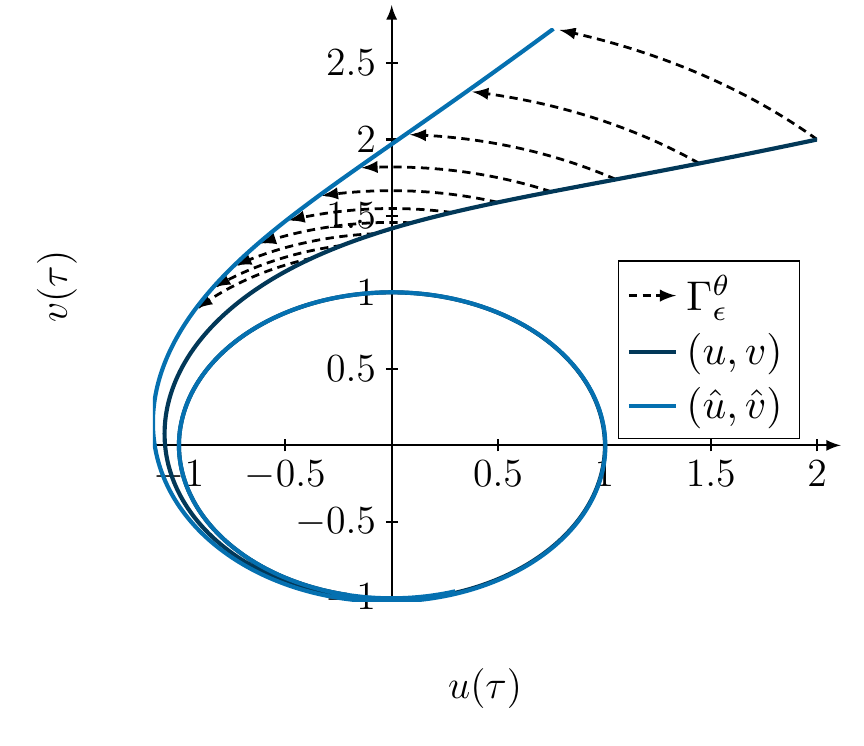
\begin{tikzpicture}
  % The axis of the plot
\begin{axis}[
    xlabel={$u(\tau)$},
    ylabel={$v(\tau)$},
    x label style={at={(axis description cs:0.5,-0.1)},anchor=north},
    y label style={at={(axis description cs:-0.1,0.55)},rotate=90,anchor=south},
    scaled x ticks = false,
    xtick={-1,-0.5,...,2},    
    %ymax = 3.22,
    %xmax = 4.5,
    legend style={at={(axis description cs:0.7,0.44)},anchor=west,nodes={scale=1.5, transform shape}},
    label style={font=\Large},
    tick label style={font=\Large},
    legend cell align={left},
    grid style=dashed,
]
\addplot[
color=black,->,>=latex,densely dashed,line width=1.0pt
]
coordinates {%
(2.0,2.0)
(1.978946794238295,2.0208338837487254)
(1.9576765381238255,2.0414461996569457)
(1.9361915782470314,2.0618346703824844)
(1.9144943307950455,2.0819970018118035)
(1.8925871371849858,2.101931018676824)
(1.8704723997145127,2.1216345347890204)
(1.8481525434478816,2.141105389404944)
(1.8256300152326046,2.1603414469321924)
(1.8029072842892586,2.1793405969922603)
(1.7799868442684372,2.1981007571785174)
(1.7568712053647004,2.2166198677943374)
(1.7335629063998106,2.2348959016804297)
(1.7100645063995694,2.2529268575283283)
(1.686378578236714,2.2707107548578858)
(1.6625077199109974,2.288245642968079)
(1.6384545488217306,2.3055295991938034)
(1.6142217024822043,2.3225607282988423)
(1.5898118390558724,2.3393371620622614)
(1.5652276343344464,2.3558570615007244)
(1.540471784820588,2.372118614613495)
(1.5155470048440667,2.388120038385831)
(1.4904560256011106,2.4038595794068005)
(1.46520159897044,2.4193355113534225)
(1.4397864953177535,2.434546136468745)
(1.414213503090457,2.4494897858505205)
(1.3884854284663455,2.4641648197040404)
(1.36260509446976,2.4785696278033393)
(1.3365753376535605,2.4927026309048523)
(1.3103990120880429,2.5065622793019857)
(1.2840789879288006,2.5201470535008585)
(1.2576181505938817,2.533455464657636)
(1.2310194003531596,2.5464860548545705)
(1.2042856520141672,2.55923739727039)
(1.1774198388147077,2.57170809174322)
(1.1504249084290281,2.5838967689711136)
(1.1233038211168125,2.5958020923656644)
(1.0960595509464197,2.607422756538551)
(1.0686950854708048,2.618757487482786)
(1.0412134254034364,2.629805042753962)
(1.01361758436451,2.640564210870318)
(0.9859105885976494,2.6510338110407683)
(0.9580954764839938,2.6612126951445894)
(0.930175298296302,2.671099747043826)
(0.9021531158789322,2.6806938827193734)
(0.8740320023263132,2.6899940504238815)
(0.8458150415667895,2.698999230604529)
(0.8175053275866855,2.7077084349508085)
(0.7891059648030166,2.716120708235827)
};
\addlegendentry{$\Gamma_{\epsilon}^{\theta}$}
\addplot[
forget plot,
color=black,->,>=latex,densely dashed,line width=1.0pt
]
coordinates {%
(1.446101254320559,1.8435702685464732)
(1.4267165181573425,1.858612425898907)
(1.407175280219362,1.8734508037324376)
(1.387479725480899,1.8880837396705226)
(1.3676320454955364,1.9025096053672652)
(1.347634389339889,1.9167268397236725)
(1.327488949450098,1.930733882833764)
(1.3071979350256557,1.9445291987479694)
(1.2867635707385643,1.9581112744528588)
(1.2661880971385764,1.9714786196709964)
(1.2454737716347979,1.9846297693672412)
(1.2246228636118153,1.9975632793942955)
(1.203637663336084,2.0102777357381565)
(1.1825204724065146,2.0227717448314424)
(1.1612736045455745,2.0350439343432907)
(1.1398993902493715,2.047092958173294)
(1.1184001729258128,2.058917495312271)
(1.0967783103586635,2.0705162489798155)
(1.0750361740246195,2.0818879470104252)
(1.0531761474478594,2.093031342786733)
(1.0312006284462667,2.1039452139691783)
(1.00911202554488,2.1146283643719332)
(0.9869127600446823,2.12507962290766)
(0.964605266871097,2.1352978431723564)
(0.9421919932475564,2.1452819041325597)
(0.9196753983826099,2.1550307102988415)
(0.8970579531570325,2.1645431918992997)
(0.8743421383934838,2.17381830542814)
(0.8515304438151647,2.1828550340119315)
(0.8286253708560586,2.1916523867566533)
(0.8056294308198786,2.2002093993255736)
(0.7825451444906864,2.2085251341329806)
(0.7593750417689777,2.2165986805311797)
(0.7361216622647785,2.224429154169486)
(0.7127875585232868,2.2320156940755407)
(0.689375289762959,2.2393574679452475)
(0.665887423354399,2.246453670735374)
(0.6423265349239325,2.253303524446081)
(0.618695208069509,2.259906278238857)
(0.5949960340914057,2.2662612084845866)
(0.5712316119615417,2.272367617685275)
(0.5474045477669138,2.2782248358781443)
(0.5235174544183424,2.283832220787353)
(0.4995729514348503,2.289189157618697)
(0.47557366466442974,2.2942950591545808)
(0.4515222260047381,2.299149365848735)
(0.4274212729097102,2.3037515451603876)
(0.4032734481782446,2.308101091890522)
(0.3790813998979738,2.3121975290690844)
};
\addplot[
forget plot,
color=black,->,>=latex,densely dashed,line width=1.0pt
]
coordinates {%
(1.0541264523851241,1.739099558958013)
(1.0358572028045212,1.7500427734835005)
(1.0174743084138842,1.7607941088208454)
(0.9989798444892525,1.7713523481853177)
(0.9803758515153417,1.7817163270796763)
(0.9616643494585884,1.7918849211516825)
(0.9428473897608713,1.8018570143606158)
(0.9239270357646295,1.8116315129433325)
(0.9049053620865853,1.8212073450792348)
(0.8857844546826823,1.8305834600746398)
(0.866566410695415,1.8397588300007541)
(0.8472533365078547,1.8487324475489484)
(0.8278473530346416,1.8575033330690651)
(0.808350587456169,1.8660705238576079)
(0.7887651770101004,1.8744330790329622)
(0.7690932698349451,1.8825900813801792)
(0.7493370226494204,1.8905406366231303)
(0.729498602536511,1.898283872644115)
(0.7095801843524283,1.905818940575944)
(0.689583952655528,1.913145013996268)
(0.6695121004270719,1.9202612894439186)
(0.6493668270888819,1.9271669871239343)
(0.6291503416181276,1.9338613497764385)
(0.6088648615861512,1.9403436430416265)
(0.5885126125015495,1.9466131557130715)
(0.5680958275233786,1.9526691998551757)
(0.547616747094178,1.9585111109322757)
(0.5270776164016487,1.9641382482533574)
(0.5064806871995613,1.9695499947831487)
(0.485828217953437,1.974745757196708)
(0.4651224728197207,1.9797249661035679)
(0.44436572131365104,1.9844870761717768)
(0.42356023797713,1.9890315662519384)
(0.40270830479770947,1.993357937637995)
(0.38181221030410123,1.9974657145789116)
(0.3608742459620506,2.0013544466187523)
(0.33989670779076625,2.0050237074010133)
(0.31888189610612616,2.0084730947416403)
(0.2978321152638741,2.0117022307020527)
(0.27674967353524754,2.0147107612732293)
(0.25563688303932114,2.017498355893237)
(0.23449605903764303,2.0200647088376145)
(0.21332951986616416,2.022409538738114)
(0.1921395866958642,2.0245325886045373)
(0.17092858328248203,2.026433625878569)
(0.1496988356910652,2.0281124423303503)
(0.1284526719143238,2.029568853291886)
(0.10719242181692065,2.030802698925862)
(0.08592041683460046,2.0318138439634774)
};
\addplot[
forget plot,
color=black,->,>=latex,densely dashed,line width=1.0pt
]
coordinates {%
(0.7500731096845435,1.6587429197626766)
(0.7326620079071562,1.6665065634197576)
(0.7151705418777214,1.6740874648147666)
(0.6976006460983029,1.6814847850547316)
(0.6799542505460318,1.6886977115377482)
(0.6622332903448885,1.695725453293337)
(0.6444397086456133,1.7025672396985834)
(0.6265754566471009,1.7092223204939514)
(0.6086424934549478,1.7156899658371387)
(0.5906427858109287,1.7219694664103433)
(0.572578307853148,1.7280601335124122)
(0.554451040461551,1.7339612992134723)
(0.5362629713976368,1.7396723163898824)
(0.5180160951442631,1.7451925588043775)
(0.49971241256220844,1.7505214212138265)
(0.4813539306784811,1.7556583194314777)
(0.4629426628535981,1.7606026899416947)
(0.44448062817259476,1.7653539904313515)
(0.42596985119420616,1.7699116998982813)
(0.40741236181458307,1.7742753186244749)
(0.3888101950480353,1.7784443682206545)
(0.37016539083806743,1.782418391339344)
(0.35147999380211803,1.7861969521134498)
(0.33275605301150035,1.7897796362096254)
(0.3139956217766445,1.7931660508236043)
(0.2952007574178178,1.7963558247067906)
(0.2763735209655852,1.7993486079043466)
(0.25751597702590995,1.8021440721693396)
(0.23863019354800857,1.8047419109775706)
(0.21971824158831857,1.807141839526438)
(0.20078219507268968,1.8093435947144)
(0.18182413053396615,1.8113469349983582)
(0.1628461269162699,1.8131516405819186)
(0.14385026537906676,1.8147575136025718)
(0.12483862904616025,1.8161643780456889)
(0.10581330276704534,1.8173720796795343)
(0.086776372825776,1.8183804855759182)
(0.06772992682538362,1.8191894850228572)
(0.04867605342886928,1.8197989893025024)
(0.029616842121155458,1.8202089316365007)
(0.01055438298034065,1.8204192672064403)
(-0.008509233551582472,1.820429973171459)
(-0.02757191689854417,1.8202410486830098)
(-0.04663157658074954,1.8198525148967888)
(-0.0656861224470777,1.8192644149406472)
(-0.08473346494884279,1.8184768127672262)
(-0.10377151532611018,1.817489794401036)
(-0.12279818583392678,1.8163034681096837)
(-0.14181138999061949,1.8149179639855704)
};
\addplot[
forget plot,
color=black,->,>=latex,densely dashed,line width=1.0pt
]
coordinates {%
(0.4992809294283036,1.5890358689295765)
(0.482613534426778,1.5941770966954647)
(0.4658931949152631,1.5991435114561887)
(0.4491217640713029,1.6039345623566765)
(0.43230108196539124,1.6085497237598456)
(0.4154329931657099,1.6129884895636601)
(0.39851934730181315,1.6172503730374226)
(0.3815619991054827,1.621334906822388)
(0.3645628082355021,1.6252416429772152)
(0.3475236390321033,1.6289701530432223)
(0.3304463602569803,1.632520028103162)
(0.313332844492856,1.6358908788518296)
(0.29618496837498187,1.6390823356377593)
(0.27900461230429197,1.642094048522933)
(0.26179366016776745,1.6449256873422393)
(0.24455399920339074,1.6475769416788237)
(0.2272875201380745,1.650047520589904)
(0.2099961164625312,1.6523371531215298)
(0.19268168435684144,1.6544455882285234)
(0.1753461225129969,1.656372594788597)
(0.15799133194850457,1.6581179615397619)
(0.14061921584348272,1.6596814969108242)
(0.12323167924912251,1.661063029437327)
(0.10583062890994815,1.6622624076595671)
(0.08841797305898896,1.6632795001438947)
(0.07099562119283655,1.6641141953703311)
(0.053565483850808546,1.6647664016536645)
(0.03612947244496496,1.6652360474791206)
(0.018689499035300088,1.6655230813910828)
(0.0012474761176449883,1.6656274719726747)
(-0.016194683585826014,1.6655492078555612)
(-0.033635067363021354,1.665288297405478)
(-0.051071762677359356,1.6648447692625963)
(-0.06850285739621005,1.664218672123177)
(-0.08592643999995528,1.6634100747485032)
(-0.10334059979620794,1.662419065533616)
(-0.12074342712472888,1.6612457529083073)
(-0.13813301356491836,1.659890265525423)
(-0.15550745214781472,1.6583527520663073)
(-0.1728648375660916,1.6566333812361662)
(-0.19020326638424156,1.6547323417567739)
(-0.20752083724894674,1.6526498423565232)
(-0.22481565109963667,1.6503861117578207)
(-0.24208581137768548,1.6479413986416014)
(-0.25932942416877447,1.6453159707326637)
(-0.27654459847914314,1.6425101156309208)
(-0.2937294464673063,1.6395241410551145)
(-0.3108820836272261,1.6363583744465824)
(-0.32800062899853377,1.6330131629216669)
};
\addplot[
forget plot,
color=black,->,>=latex,densely dashed,line width=1.0pt
]
coordinates {%
(0.283677298722318,1.5226291721826193)
(0.2677171200926778,1.5255162894570995)
(0.2517275632348438,1.5282361204191548)
(0.23571040211984967,1.5307883629550902)
(0.2196673927039804,1.5331727373020865)
(0.20360029426898527,1.5353889819834543)
(0.1875108686158608,1.537436853975828)
(0.17140088011390858,1.539316128704833)
(0.15527209550341123,1.541026600072748)
(0.13912628367104893,1.5425680804905573)
(0.12296521535908517,1.543940400900092)
(0.10679066266883536,1.5451434107796798)
(0.0906043992905363,1.546176978208033)
(0.07440820015993395,1.547040989882175)
(0.05820384122215878,1.5477353511439673)
(0.04199309941739536,1.5482599858679296)
(0.025777752629399565,1.5486148363751773)
(0.009559579047990777,1.548799863759309)
(-0.006659642846105176,1.5488150477748086)
(-0.02287813447574079,1.5486603868504876)
(-0.03909411729100637,1.548335897896508)
(-0.05530581299573215,1.54784161640044)
(-0.07151144379475333,1.5471775965816708)
(-0.08770923255747423,1.5463439113105788)
(-0.10389740301281086,1.5453406521002102)
(-0.12007417994534436,1.544167928866704)
(-0.1362377893890227,1.5428258701578048)
(-0.1523864588219793,1.5413146231680792)
(-0.16851841736171153,1.5396343536855726)
(-0.18463189595791438,1.5377852460264785)
(-0.20072512758228228,1.5357675028784044)
(-0.21679634742843676,1.533581345448828)
(-0.232843793108507,1.5312270135126491)
(-0.24886570484523868,1.5287047653250185)
(-0.26486032564471484,1.5260148774058553)
(-0.28082590146994413,1.5231576443311126)
(-0.2967606815053748,1.5201333793769403)
(-0.31266291831837517,1.5169424141943855)
(-0.32853086805138537,1.5135850987708692)
(-0.3443627906154163,1.510061801402913)
(-0.36015694988344116,1.506372908666462)
(-0.37591161388368144,1.502518825384804)
(-0.3916250549927856,1.4984999745940886)
(-0.40729555011951746,1.4943167974579552)
(-0.4229213806953128,1.4899697521825193)
(-0.4385008331017989,1.485459315187027)
(-0.4540321988750681,1.4807859811192756)
(-0.4695137748314589,1.4759502624636653)
(-0.48494386325663175,1.4709526894744005)
};
\addplot[
forget plot,
color=black,->,>=latex,densely dashed,line width=1.0pt
]
coordinates {%
(0.09319363131665603,1.4551819451667813)
(0.07795018759584359,1.4560780592762008)
(0.06269817725540085,1.4568144991975118)
(0.047439292540995666,1.4573911829038912)
(0.03217520557391805,1.457808047250733)
(0.01690759021344651,1.4580650465169613)
(0.0016381206002845303,1.4581621525170043)
(-0.01363152879538191,1.4580993545983973)
(-0.028899683383295384,1.4578766596461894)
(-0.044164668659433665,1.4574940920878052)
(-0.0594248105351843,1.4569516938707427)
(-0.07467843568973849,1.4562495244356952)
(-0.0899238714160815,1.455387660789486)
(-0.1051594459646654,1.4543661974799091)
(-0.12038348874691207,1.4531852465948563)
(-0.1355943302035012,1.4518449375884088)
(-0.15079030217574707,1.4503454173717096)
(-0.16596973826843708,1.4486868503993398)
(-0.1811309739193772,1.4468694186013336)
(-0.19627234657267467,1.4448933213491808)
(-0.21139219575929735,1.4427587752383462)
(-0.22648886340341862,1.4404660143175712)
(-0.24156069398814017,1.4380152900399141)
(-0.2566060347243256,1.4354068712199473)
(-0.27162323572378383,1.4326410439314599)
(-0.28661065016741805,1.429718111360206)
(-0.30156663451635557,1.4266383940404492)
(-0.3164895486830683,1.4234022297342448)
(-0.3313777562089724,1.4200099733772673)
(-0.3462296244370077,1.4164619969924777)
(-0.36104352467178563,1.4127586895210553)
(-0.37581783240640665,1.4089004570970447)
(-0.390550927481451,1.4048877228705792)
(-0.40524119425376814,1.4007209269241354)
(-0.4198870216810221,1.3964005258157877)
(-0.43448680364762715,1.3919269931887592)
(-0.4490389391143445,1.3873008196009315)
(-0.4635418322776679,1.382522512396976)
(-0.47799389274808135,1.377592595663267)
(-0.4923935357279642,1.3725116101805943)
(-0.5067391821891414,1.3672801133746748)
(-0.5210292590500816,1.3618986792644647)
(-0.5352621993527408,1.3563678984082728)
(-0.5494364423553796,1.3506883775831457)
(-0.5635504334412651,1.3448607388811122)
(-0.5776026248180675,1.3388856213040456)
(-0.5915914755071885,1.3327636801126337)
(-0.6055154514807396,1.3264955866410482)
(-0.6193730258310068,1.320082028213232)
};
\addplot[
forget plot,
color=black,->,>=latex,densely dashed,line width=1.0pt
]
coordinates {%
(-0.07798193781933803,1.3840144606983118)
(-0.09247074577510381,1.383121965417238)
(-0.10694943119048762,1.3820777942142028)
(-0.1214163873779421,1.3808820626506055)
(-0.13587002889070957,1.3795349018137306)
(-0.15030877073801996,1.3780364594273873)
(-0.1647310296750618,1.3763868997942426)
(-0.17913522415177438,1.374586403801591)
(-0.19351977449624047,1.3726351689029317)
(-0.20788310311587777,1.370533409098103)
(-0.22222363474797638,1.3682813548926076)
(-0.23653979690898394,1.3658792531902015)
(-0.25083001970026986,1.3633273674015784)
(-0.26509273610432593,1.3606259773883655)
(-0.27932638219961736,1.3577753794344334)
(-0.2935293971874744,1.3547758861589398)
(-0.3077002233318588,1.3516278263945876)
(-0.321837306640263,1.3483315453617848)
(-0.33593909685112594,1.3448874045659265)
(-0.3500040475999723,1.3412957817660351)
(-0.3640306165097569,1.3375570708154125)
(-0.37801726534620794,1.3336716816022687)
(-0.3919624603180327,1.3296400402131494)
(-0.40586467218717215,1.3254625888042144)
(-0.4197223764390102,1.3211397855633644)
(-0.43353405340661605,1.3166721044812424)
(-0.4472981884642221,1.3120600354095668)
(-0.4610132722227644,1.3073040841280181)
(-0.47467780068110704,1.3024047722272187)
(-0.48829027538555747,1.2973626370317863)
(-0.5018492035651925,1.2921782314377852)
(-0.515353098301875,1.2868521238729447)
(-0.5288004787499161,1.2813848984325507)
(-0.542189870270982,1.2757771547154213)
(-0.5555198045751085,1.2700295077027814)
(-0.5687888197338036,1.2641425872873349)
(-0.5819954605993901,1.258117038911619)
(-0.5951382789035964,1.2519535233297918)
(-0.6082158333938996,1.2456527164721503)
(-0.6212266899960874,1.2392153093808582)
(-0.6341694219762205,1.2326420081436429)
(-0.6470426101019982,1.2259335338254602)
(-0.659844842803528,1.219090622398126)
(-0.6725747163334957,1.2121140246679165)
(-0.6852308348865711,1.2050045061152266)
(-0.6978118102556443,1.1977628457428895)
(-0.7103162626701022,1.1903898374517836)
(-0.7227428208808215,1.182886289804634)
(-0.7350901221821204,1.1752530256542235)
};
\addplot[
forget plot,
color=black,->,>=latex,densely dashed,line width=1.0pt
]
coordinates {%
(-0.23322791946942856,1.3074599868720134)
(-0.2469065525934838,1.3049459889132526)
(-0.260558126588295,1.3022888859255641)
(-0.2741811280909272,1.299488972145278)
(-0.2877740625430876,1.2965465547550155)
(-0.3013354393312312,1.2934619564263878)
(-0.3148637714145058,1.2902355153854812)
(-0.32835757530872967,1.286867585431159)
(-0.34181537119666794,1.2833585359088961)
(-0.3552356831356839,1.2797087516635293)
(-0.36861703923489186,1.275918632998218)
(-0.3819579721101178,1.2719885954972354)
(-0.3952570188503175,1.2679190700882215)
(-0.4085127211034355,1.2637105030458904)
(-0.4217236253424703,1.25936335590741)
(-0.4348882830366254,1.2548781054274152)
(-0.44800525041150335,1.2502552434170244)
(-0.4610730889045946,1.2454952767791108)
(-0.47409036549671535,1.2405987275085606)
(-0.487055652739828,1.2355661326068303)
(-0.49996752891867413,1.2303980440318663)
(-0.5128245780575663,1.225095028459104)
(-0.5256253901784722,1.2196576673490678)
(-0.5383685615334963,1.214086556983734)
(-0.5510526947077897,1.2083823083448022)
(-0.5636763987767023,1.2025455470568136)
(-0.5762382893844992,1.1965769131245185)
(-0.5887369889447116,1.190477060989308)
(-0.6011711268390346,1.1842466595818377)
(-0.6135393395421711,1.1778863921803944)
(-0.6258402707626355,1.1713969563152224)
(-0.6380725715772463,1.1647790636581226)
(-0.6502349005071407,1.1580334397755834)
(-0.6623259238264113,1.1511608244247695)
(-0.6743443156404825,1.1441619713121645)
(-0.6862887580380337,1.1370376480243682)
(-0.6981579410321573,1.1297886355567317)
(-0.7099505628776066,1.1224157285587937)
(-0.7216653303578251,1.1149197355218077)
(-0.7333009588147037,1.1073014784754274)
(-0.7448561722951419,1.099561792906811)
(-0.7563297036967866,1.0917015276778652)
(-0.7677202949129492,1.0837215449406243)
(-0.7790266969766997,1.0756227200507724)
(-0.7902476702041388,1.0674059414792998)
(-0.801381984336848,1.0590721107223002)
(-0.8124284184829793,1.0506221418980095)
(-0.8233857607570257,1.0420569608761256)
(-0.8342528095160386,1.0333775068815128)
};
\addplot[
forget plot,
color=black,->,>=latex,densely dashed,line width=1.0pt
]
coordinates {%
(-0.37445604602258903,1.2245267732124638)
(-0.38725847754100234,1.2205384141032145)
(-0.40001845520783474,1.2164162051930645)
(-0.4127345698389973,1.2121606014163828)
(-0.42540542347104887,1.2077720705622406)
(-0.4380296266067922,1.2032510938966532)
(-0.450605794951828,1.198598167151146)
(-0.46313254947595534,1.1938138005328043)
(-0.4756085164291459,1.1888985187162793)
(-0.48803232755829545,1.183852860764755)
(-0.5004026202650478,1.17867738007439)
(-0.5127180378993687,1.17337264422842)
(-0.524977230065374,1.1679392348431061)
(-0.5371788524232384,1.1623777477490294)
(-0.5493215670049572,1.156688792830429)
(-0.5614040423867827,1.1508729939599194)
(-0.5734249537398334,1.1449309889166837)
(-0.5853829825556954,1.1388634292490156)
(-0.5972768174648225,1.1326709803239847)
(-0.6091051542024822,1.1263543212311327)
(-0.6208666957198428,1.1199141447110226)
(-0.6325601523158406,1.1133511570715888)
(-0.6441842415694407,1.1066660779098225)
(-0.6557376887264046,1.099859640276707)
(-0.6672192268309969,1.0929325905934086)
(-0.6786275968307313,1.0858856885411772)
(-0.689961547718861,1.0787197069861594)
(-0.7012198365581508,1.0714354316825865)
(-0.7124012287031577,1.064033661346543)
(-0.7235044979948012,1.05651520767801)
(-0.7345284268584031,1.0488808952026967)
(-0.7454718064441068,1.0411315611929883)
(-0.756333436671698,1.0332680554272404)
(-0.7671121263866315,1.0252912401371184)
(-0.7778066935707056,1.017201990047347)
(-0.7884159654695029,1.0090011922747124)
(-0.7989387787049549,1.0006897462019098)
(-0.809373979284816,0.9922685632122535)
(-0.8197204225643068,0.9837385663564245)
(-0.8299769738866531,0.9751006909803241)
(-0.8401425084922358,0.9663558843170165)
(-0.850215911633214,0.9575051053693919)
(-0.8601960787026622,0.9485493248131487)
(-0.8700819153626874,0.9394895248980931)
(-0.8798723376715251,0.9303266993477594)
(-0.8895662722096146,0.9210618532573475)
(-0.8991626562046555,0.9116960029899814)
(-0.9086604376556406,0.902230176071286)
(-0.9180585748381083,0.892665410360781)
};
\addplot[
color=theta_1,line width=1.5pt,
]
coordinates {%
(2.0,2.0)
(1.8909237144620223,1.9682726491844558)
(1.7896932832135488,1.93922916589428)
(1.6953480903861957,1.9125154277625709)
(1.6070772150424197,1.8878318291790523)
(1.5241913742499995,1.8649230698181607)
(1.446101254320559,1.8435702685464732)
(1.3723000282364406,1.8235846012500532)
(1.302349524824366,1.8048022682108587)
(1.2358691344755055,1.787080457614985)
(1.1725266962242977,1.7702940304257995)
(1.1120311492122734,1.75433284760152)
(1.0541264523851241,1.739099558958013)
(0.9985865610130982,1.724507776798649)
(0.9452112438244539,1.7104805555526224)
(0.8938225751884632,1.696949117168299)
(0.8442619942566421,1.6838517829011135)
(0.7963878144428987,1.6711330690329982)
(0.7500731096845435,1.6587429197626766)
(0.7052039107516748,1.646636052950034)
(0.6616776588375324,1.634771399517656)
(0.619401882510735,1.6231116241458827)
(0.5782930482848065,1.6116227091864976)
(0.5382755664788164,1.6002735950835452)
(0.4992809294283036,1.5890358689295765)
(0.46124695739202526,1.5778834922428373)
(0.42411714251912414,1.5667925644192604)
(0.3878400708810182,1.555741114586365)
(0.35236891240075735,1.5447089181327596)
(0.31766097353103656,1.5336773360819524)
(0.283677298722318,1.5226291721826193)
(0.2503823267825255,1.5115485499618961)
(0.21774356479859394,1.5004207961783331)
(0.18573132033609682,1.489232345428381)
(0.15431844456542215,1.4779706486642115)
(0.12348011460558986,1.466624096013874)
(0.09319363131665603,1.4551819451667813)
(0.06343823778415264,1.4436342572712486)
(0.03419496092366535,1.4319718412043814)
(0.005446460851494486,1.4201862006106063)
(-0.022823098533800674,1.4082694886555749)
(-0.050628170862434534,1.3962144656760038)
(-0.07798193781933803,1.3840144606983118)
(-0.10489640163225414,1.371663339506448)
(-0.1313824854660229,1.3591554697974326)
(-0.15745010763627187,1.346485695808486)
(-0.18310826272498038,1.3336493103343394)
(-0.20836508559274716,1.32064203298008)
(-0.23322791946942856,1.3074599868720134)
(-0.25770337030057433,1.2940996803113927)
(-0.28179736349352497,1.2805579875119746)
(-0.30551519067052724,1.2668321329260661)
(-0.3288615575604617,1.2529196750735312)
(-0.3518406242898626,1.2388184931104211)
(-0.37445604602258903,1.2245267732124638)
(-0.39671100796823033,1.2100429969480764)
(-0.418608260981142,1.195365929356747)
(-0.44015014979191625,1.1804946096851487)
(-0.46133864141650105,1.1654283419968436)
(-0.4821753601442236,1.1501666833273516)
(-0.5026616038385809,1.1347094385839611)
(-0.5227983717073538,1.1190566511616133)
(-0.542586388345061,1.1032085948579187)
(-0.5620261193206268,1.087165768881601)
(-0.581117796191324,1.0709288892907114)
(-0.5998614322284461,1.0544988837760927)
(-0.6182568386451427,1.0378768861989545)
(-0.6363036446569481,1.02106422967163)
(-0.6540013090956095,1.0040624426463909)
(-0.6713491366017438,0.9868732432482351)
(-0.6883462924405092,0.9694985340410522)
(-0.7049918129880477,0.9519403983517473)
(-0.721284620505071,0.9342010949232102)
(-0.7372235337638698,0.916283054025143)
(-0.7528072787787248,0.898188873453049)
(-0.7680345015226597,0.8799213137129367)
(-0.7829037748948716,0.8614832952883578)
(-0.7974136080995439,0.8428778949255221)
(-0.8115624596896841,0.8241083405322891)
(-0.8253487455198963,0.8051780078566636)
(-0.8387708434350303,0.7860904182815868)
(-0.8518271027895983,0.7668492347893756)
(-0.8645158554824741,0.7474582572369596)
(-0.8768354191910334,0.7279214205415006)
(-0.8887841045291665,0.7082427912855154)
(-0.900360223674063,0.6884265637431564)
(-0.9115620970566775,0.6684770565382654)
(-0.9223880570416841,0.6483987103089582)
(-0.9328364546615934,0.6281960842241916)
(-0.9429056672601397,0.6078738521449197)
(-0.9525941018254681,0.5874368001938859)
(-0.961900200107047,0.5668898236579726)
(-0.9708224445229195,0.5462379235405835)
(-0.9793593635015687,0.5254862032479114)
(-0.9875095345034712,0.5046398660478608)
(-0.9952715889081998,0.4837042117947846)
(-1.0026442173801364,0.4626846334798449)
(-1.009626172928081,0.44158661444468217)
(-1.0162162746389873,0.42041572533205934)
(-1.0224134120978001,0.39917762077734176)
(-1.0282165494704487,0.3778780361515153)
(-1.03362472736247,0.35652278491937034)
(-1.0386370665097941,0.33511775539762056)
(-1.043252770732908,0.3136689076834989)
(-1.0474711324004387,0.29218226989993157)
(-1.0512915342670381,0.2706639353244593)
(-1.054713450419874,0.24912005970322637)
(-1.0577364497988118,0.22755685786458435)
(-1.060360198709603,0.20598060055491452)
(-1.0625844651704264,0.1843976108592958)
(-1.064409119265137,0.16281426141510924)
(-1.0658341351670781,0.14123697124424936)
(-1.0668595934612797,0.11967220248843272)
(-1.0674856833364592,0.0981264571883857)
(-1.0677127058057712,0.07660627397741128)
(-1.067541073487306,0.055118224992918186)
(-1.066971312672999,0.033668912616763816)
(-1.0660040649001794,0.012264966233656208)
(-1.0646400888346945,-0.009086960944637942)
(-1.0628802621009548,-0.030380195054293728)
(-1.0607255812690937,-0.05160804496783574)
(-1.0581771634306387,-0.07276380548530828)
(-1.0552362471986325,-0.09384076058635504)
(-1.051904194280674,-0.1148321864904165)
(-1.048182490086036,-0.13573135496843333)
(-1.0440727439963067,-0.1565315367254811)
(-1.0395766902680839,-0.1772260045764494)
(-1.034696188614351,-0.19780803667372612)
(-1.029433225309756,-0.21827091936340304)
(-1.0237899130062378,-0.23860795075699398)
(-1.0177684909965576,-0.25881244397722747)
(-1.0113713255343366,-0.2788777303125095)
(-1.0046009101214977,-0.2987971622863737)
(-0.9974598661958797,-0.3185641163000936)
(-0.9899509420359709,-0.3381719967276041)
(-0.9820770129247062,-0.357614238844264)
(-0.973841080980426,-0.37688431195975425)
(-0.9652462748307185,-0.3959757226038439)
(-0.9562958492704987,-0.41488201763201155)
(-0.9469931866405193,-0.43359678549996034)
(-0.9373417945795355,-0.4521136610992699)
(-0.9273453050838736,-0.47042632917848404)
(-0.9170074743334531,-0.48852852689518167)
(-0.906332181915522,-0.5064140468794138)
(-0.8953234299626515,-0.5240767402875632)
(-0.8839853431610472,-0.5415105186624158)
(-0.872322168078794,-0.5587093565198122)
(-0.8603382703664277,-0.5756672964549548)
(-0.8480381344703359,-0.5923784510204333)
(-0.8354263624368702,-0.6088370056147578)
(-0.8225076726296141,-0.6250372213626855)
(-0.8092868987267376,-0.6409734375173902)
(-0.7957689898355375,-0.6566400723116845)
(-0.7819590067367842,-0.6720316286499182)
(-0.7678621209886045,-0.687142696016003)
(-0.7534836134976085,-0.7019679529449888)
(-0.7388288728518734,-0.7165021696806264)
(-0.7239033936328194,-0.7307402107424608)
(-0.708712776236833,-0.7446770354895114)
(-0.6932627236601954,-0.758307702361735)
(-0.6775590392072728,-0.7716273718509394)
(-0.6616076250293585,-0.7846313083168803)
(-0.6454144801070023,-0.797314882381924)
(-0.6289856981644659,-0.809673573293677)
(-0.6123274665321471,-0.8217029701570872)
(-0.5954460645024625,-0.8333987736088717)
(-0.5783478590089663,-0.8447568002810821)
(-0.5610393033335392,-0.8557729838847835)
(-0.5435269347957187,-0.8664433772889858)
(-0.5258173723667178,-0.8767641545755847)
(-0.5079173145488597,-0.8867316127496045)
(-0.48983353896926857,-0.8963421717497873)
(-0.4715728968114412,-0.9055923791903233)
(-0.45314231130820676,-0.9144789112078877)
(-0.4345487752325816,-0.9229985741493637)
(-0.4157993482616244,-0.9311483062818597)
(-0.39690115433622725,-0.9389251794194855)
(-0.37786138102805095,-0.9463263989425174)
(-0.35868727507953485,-0.9533493066300499)
(-0.3393861389999594,-0.9599913826054203)
(-0.3199653289969226,-0.966250246182489)
(-0.300432252160571,-0.9721236571909132)
(-0.2807943636125177,-0.9776095172406768)
(-0.26105916362127396,-0.9827058709243005)
(-0.24123419545842056,-0.9874109065681582)
(-0.22132704336184827,-0.9917229568497201)
(-0.20134532738151498,-0.9956405008956599)
(-0.18129670143622797,-0.9991621646893872)
(-0.1611888504414942,-1.0022867218615876)
(-0.141029487386072,-1.0050130944233813)
(-0.120826350400216,-1.0073403534198995)
(-0.10058719965950227,-1.009267719746888)
(-0.08031981284450798,-1.0107945671062164)
(-0.060031984047740274,-1.0119204195568148)
(-0.03973152053736869,-1.0126449522864622)
(-0.0194262394265082,-1.0129679924459234)
(0.0008760353652652042,-1.0128895194507466)
(0.02116747615303956,-1.0124096652074184)
(0.04144025452847133,-1.0115287142627873)
(0.06168654529237649,-1.0102471050867106)
(0.08189852937854447,-1.008565429909954)
(0.10206839587860159,-1.006484433267973)
(0.12218834573949891,-1.0040050127441391)
(0.14225059486236455,-1.0011282188295867)
(0.1622473771994029,-0.9978552547114092)
(0.18217094784735768,-0.9941874759886804)
(0.2020135861944614,-0.9901263905519118)
(0.22176759921994865,-0.9856736590322182)
(0.24142532423445529,-0.9808310929468191)
(0.26097913206276346,-0.9756006545973143)
(0.2804214301351311,-0.9699844565670138)
(0.2997446655462298,-0.9639847610615712)
(0.31894132810204756,-0.9576039791806538)
(0.3380039533487982,-0.9508446701376684)
(0.3569251254080527,-0.9437095410888859)
(0.3756974801219608,-0.9362014456550333)
(0.39431370808610305,-0.9283233827323469)
(0.4127665575417945,-0.920078495694499)
(0.4310488373085474,-0.9114700712943182)
(0.44915341969337175,-0.9025015385000137)
(0.46707324337543776,-0.893176467265914)
(0.4848013163999618,-0.8834985674950423)
(0.5023307191704259,-0.8734716879854555)
(0.5196546068663555,-0.8630998142738171)
(0.5367662124007655,-0.8523870674978149)
(0.5536588491867283,-0.8413377028908299)
(0.5703259138653817,-0.8299561082013411)
(0.5867608890012661,-0.818246802051063)
(0.602957345753239,-0.8062144322952639)
(0.6189089465981024,-0.7938637749029095)
(0.6346094478070425,-0.7811997313891522)
(0.6500527020144145,-0.7682273270472161)
(0.6652326607534155,-0.7549517091619115)
(0.6801433769333327,-0.7413781450471758)
(0.6947790072752593,-0.7275120200281117)
(0.7091338147049366,-0.7133588353679243)
(0.7232021708560508,-0.6989242064594788)
(0.7369785583924583,-0.6842138606826665)
(0.7504575731003716,-0.6692336348296357)
(0.7636339262156258,-0.6539894730614132)
(0.7765024466115878,-0.6384874246259291)
(0.7890580829388559,-0.6227336415279466)
(0.8012959056515676,-0.6067343759738311)
(0.8132111090835298,-0.5904959780484109)
(0.8247990134629216,-0.5740248933188825)
(0.8360550668233003,-0.5573276602522694)
(0.8469748468826341,-0.5404109076496425)
(0.8575540628843299,-0.5232813520629374)
(0.8677885576203876,-0.5059457955323754)
(0.8776743089287375,-0.48841112256787744)
(0.8872074313609994,-0.4706842974381339)
(0.8963841778543293,-0.4527723615162755)
(0.9052009412968697,-0.4346824305161801)
(0.9136542560443024,-0.4164216916913294)
(0.9217407994240155,-0.3979974009777447)
(0.9294573930636697,-0.3794168801663853)
(0.9368010042385898,-0.3606875140044497)
(0.9437687471518459,-0.34181674727089356)
(0.9503578841464537,-0.3228120818269719)
(0.9565658269054335,-0.3036810736857003)
(0.962390137677457,-0.28443133013662414)
(0.9678285301041335,-0.2650705065391343)
(0.972878870263539,-0.2456063033494315)
(0.9775391775904451,-0.2260464630717424)
(0.9818076257240094,-0.20639876718213032)
(0.9856825433509094,-0.18667103305962163)
(0.9891624149834196,-0.16687111090010434)
(0.9922458814850124,-0.1470068805338801)
(0.9949317407250967,-0.12708624831236182)
(0.9972189481120285,-0.1071171439575189)
(0.9991066170583576,-0.08710751739872424)
(1.0005940195087335,-0.06706533565478817)
(1.0016805862662637,-0.046998579648499815)
(1.0023659071408013,-0.026915240965273257)
(1.002649731231657,-0.006823318692319863)
(1.0025319670742725,0.013269183777011518)
(1.0020126827229274,0.03335426194183458)
(1.0010921058964108,0.05342391336554851)
(0.999770623845725,0.07347014089566875)
(0.9980487831972586,0.09348495587370334)
(0.9959272898158148,0.11346038132381495)
(0.9934070085607123,0.13338845514721903)
(0.9904889629875986,0.15326123330984265)
(0.9871743351365344,0.17307079299747263)
(0.9834644649458255,0.19280923581712958)
(0.9793608497567059,0.2124686909624472)
(0.9748651437806078,0.23204131836400343)
(0.9699791574721424,0.25151931183317255)
(0.9647048568793029,0.27089490219605383)
(0.9590443629422355,0.2901603604142676)
(0.9529999505697169,0.3093080006799239)
(0.9465740478034884,0.3283301835040887)
(0.9397692348767136,0.34721931878453893)
(0.9325882432126161,0.36596786885437005)
(0.9250339544925444,0.38456835151509494)
(0.9171093994254002,0.4030133430389599)
(0.9088177565390272,0.42129548115131943)
(0.900162350966438,0.4394074679907078)
(0.8911466531384009,0.4573420730419582)
(0.8817742774520877,0.47509213605193285)
(0.8720489809267717,0.4926505699293534)
(0.8619746615913297,0.5100103635615453)
(0.8515553569916677,0.527164584646835)
(0.8407952425978112,0.544106382484441)
(0.829698630150849,0.5608289907309458)
(0.8182699660614048,0.5773257301551807)
(0.8065138295855742,0.5935900113083106)
(0.7944349309651021,0.6096153371635328)
(0.7820381095926047,0.6253953057421521)
(0.7693283320879846,0.6409236126906944)
(0.7563106903480833,0.6561940538307696)
(0.7429903996142359,0.6712005277010878)
(0.7293727962673244,0.685937037954698)
(0.715463335742254,0.7003976957928477)
(0.7012675903615757,0.7145767223405854)
(0.6867912471130193,0.72846845097425)
(0.672040105464454,0.742067329653172)
(0.6570200750261265,0.7553679231429546)
(0.6417371731313722,0.7683649151704353)
(0.6261975224723064,0.7810531105885427)
(0.6104073486544029,0.793427437470048)
(0.5943729777241582,0.8054829491633894)
(0.578100833731591,0.8172148263561213)
(0.5615974360534685,0.8286183789348426)
(0.5448693968124512,0.8396890478961546)
(0.5279234182428734,0.8504224071929033)
(0.5107662900086879,0.8608141655182784)
(0.49340488657797416,0.8708601681239917)
(0.47584616445694267,0.8805563984822667)
(0.45809715928683736,0.8898989797930944)
(0.44016498308959884,0.8988841766083053)
(0.4220568214150367,0.9075083963342276)
(0.40377993045553456,0.9157681906742566)
(0.3853416341291782,0.9236602570103715)
(0.3667493212028797,0.9311814397972814)
(0.34801044273613774,0.9383287322635254)
(0.32913250850682296,0.945099277004655)
(0.3101230841318283,0.9514903672746083)
(0.2909897880891672,0.9574994481359007)
(0.2717402886586081,0.9631241174847621)
(0.252382300839734,0.9683621270115048)
(0.23292358324846285,0.9732113830953116)
(0.21337193525238363,0.9776699480187716)
(0.19373519377586346,0.9817360406526148)
(0.17402122986512059,0.9854080367425913)
(0.15423794569503854,0.9886844698112406)
(0.13439327139509494,0.9915640317452183)
(0.11449516186204883,0.994045573315466)
(0.09455159356051188,0.9961281046295485)
(0.07457056136678392,0.9978107956206598)
(0.054560075642617265,0.9990929769320621)
(0.034528158598746056,0.9999741393728069)
(0.014482841176406441,1.0004539343212882)
(-0.005567840139586416,1.0005321739377584)
(-0.025615846549350618,1.0002088312349875)
(-0.045653140168738594,0.9994840400803637)
(-0.06567168726114955,0.9983580951292368)
(-0.08566346132389852,0.9968314521538733)
(-0.1056204463598251,0.9949047277052885)
(-0.12553464024117644,0.9925786984011237)
(-0.14539805783636284,0.9898543008896079)
(-0.16520273421729822,0.9867326314683034)
(-0.18494072785937996,0.9832149456348137)
(-0.20460412383283474,0.9793026575691454)
(-0.2241850369636326,0.9749973396718855)
(-0.24367561490247572,0.9703007225226146)
(-0.26306804142691254,0.9652146932820557)
(-0.2823545395413208,0.9597412951660352)
(-0.3015273745874164,0.9538827266953824)
(-0.320578857350246,0.9476413408049773)
(-0.33950134714600494,0.9410196438866449)
(-0.35828725489040186,0.9340202947666532)
(-0.3769290461439406,0.9266461041246193)
(-0.39541924413833396,0.9189000331541053)
(-0.4137504327806673,0.91078519191793)
(-0.4319152596295489,0.9023048383773973)
(-0.4499064388466155,0.8934623770763961)
(-0.4677167541207994,0.8842613577627442)
(-0.48533906156407886,0.8747054739468492)
(-0.5027662925954658,0.8647985615307107)
(-0.5199914568568528,0.8545445978379046)
(-0.5370076448968867,0.8439476991120961)
(-0.5538080309779355,0.8330121191073037)
(-0.5703858758243848,0.8217422474415916)
(-0.5867345293259297,0.8101426078243205)
(-0.6028474332038718,0.7982178562256065)
(-0.6187181236395144,0.7859727789894262)
(-0.634340233973308,0.7734122912639224)
(-0.6497074972306245,0.7605414349245364)
(-0.6648137485516845,0.7473653762577526)
(-0.6796529277209622,0.7338894040733264)
(-0.6942190816030619,0.7201189275941454)
(-0.7085063665347807,0.706059474292421)
(-0.7225090506624053,0.6917166874655106)
(-0.7362215162497021,0.6770963241133869)
(-0.7496382619351089,0.6622042526889188)
(-0.7627539049342592,0.6470464506641851)
(-0.7755631831961419,0.6316290021123938)
(-0.7880609575193612,0.6159580952734868)
(-0.8002422137585626,0.6000400204897068)
(-0.8121020646954452,0.583881167263745)
(-0.8236357519974825,0.5674880216873542)
(-0.8348386481566394,0.5508671639276285)
(-0.8457062583452136,0.5340252655899389)
(-0.8562342222296901,0.5169690870357908)
(-0.8664183158054113,0.49970547461740983)
(-0.8762544529890728,0.4822413579905137)
(-0.8857386872762162,0.4645837473173273)
(-0.8948672133343261,0.4467397304394393)
(-0.9036363685263994,0.4287164700239252)
(-0.9120426344068864,0.41052120072316073)
(-0.9200826382403573,0.3921612264238726)
(-0.9277531541955091,0.3736439170815504)
(-0.9350511046855797,0.35497670582869384)
(-0.9419735616099912,0.336167086001912)
(-0.9485177475253366,0.31722260813103037)
(-0.9546810367997569,0.29815087692523645)
(-0.9604609567396667,0.27895954825253894)
(-0.9658551884359264,0.25965632599727295)
(-0.9708615677461109,0.2402489589893083)
(-0.9754780861619062,0.22074523789055917)
(-0.9797028916083814,0.20115299206177376)
(-0.9835342892674906,0.18148008647061942)
(-0.9869707423027367,0.16173441856252385)
(-0.9900108723099288,0.14192391498181295)
(-0.992653459941899,0.12205652843623586)
(-0.9948974453944591,0.10214023450284657)
(-0.9967419288254588,0.08218302842349827)
(-0.9981861708114678,0.06219292192156636)
(-0.9992295926198859,0.042177939977441695)
(-0.9998717763440808,0.022146117577832143)
(-1.0001124651192435,0.002105496502659933)
(-0.9999515632192674,-0.017935877906398705)
(-0.9993891360893356,-0.03796995997856781)
(-0.9984254104512461,-0.05798870690087739)
(-0.9970607741276019,-0.07798408197567376)
(-0.9952957758292833,-0.09794805786607633)
(-0.9931311249761249,-0.11787261980476353)
(-0.9905676914081288,-0.13774976881216652)
(-0.987606505053596,-0.1575715249091585)
(-0.9842487555830314,-0.1773299303237955)
(-0.9804957918242695,-0.1970170526841643)
(-0.9763491212487372,-0.21662498820527018)
(-0.9718104093652071,-0.23614586486381686)
(-0.9668814790440338,-0.2555718455601246)
(-0.9615643098931511,-0.27489513125332415)
(-0.9558610374093226,-0.294107964098693)
(-0.9497739520508444,-0.31320263056989034)
(-0.9433054983577703,-0.33217146455105934)
(-0.9364582739650713,-0.3510068504143502)
(-0.9292350285753899,-0.3697012260808503)
(-0.9216386629438942,-0.38824708607264524)
(-0.9136722275850728,-0.40663698450482544)
(-0.9053389215774104,-0.42486353808075056)
(-0.8966420912815531,-0.4429194290575536)
(-0.887585228989461,-0.4607974081835917)
(-0.8781719716076903,-0.4784902976234483)
(-0.8684060991704476,-0.4959909938357966)
(-0.8582915332428833,-0.5132924704127009)
(-0.8478323353850794,-0.5303877809068855)
(-0.8370327055154443,-0.547270061619303)
(-0.8258969802355371,-0.563932534359344)
(-0.8144296311849296,-0.5803685091999823)
(-0.8026352631175401,-0.5965713871199811)
(-0.7905186120762562,-0.6125346626618654)
(-0.7780845434968261,-0.6282519265459429)
(-0.7653380502472147,-0.6437168682411593)
(-0.7522842506909254,-0.6589232785287755)
(-0.7389283866280757,-0.6738650519941194)
(-0.7252758211027531,-0.6885361894400135)
(-0.7113320362885556,-0.7029308003123127)
(-0.697102631281816,-0.7170431050622499)
(-0.6825933198596987,-0.7308674374713096)
(-0.6678099282768499,-0.7443982469816158)
(-0.652758392813788,-0.7576301008571529)
(-0.637444757407378,-0.7705576863737672)
(-0.6218751712315962,-0.7831758129568465)
(-0.6060558862221752,-0.7954794142613122)
(-0.5899932546230886,-0.8074635502485313)
(-0.5736937264470102,-0.8191234091784195)
(-0.5571638467840792,-0.8304543094663244)
(-0.5404102532155307,-0.8414517015936965)
(-0.5234396731419704,-0.8521111699295856)
(-0.5062589210734312,-0.8624284344964177)
(-0.48887489598149125,-0.8723993527671112)
(-0.47129457853278356,-0.8820199213317674)
(-0.4535250281539173,-0.8912862773879126)
(-0.4355733802574593,-0.9001947003446299)
(-0.41744684337182963,-0.9087416133110415)
(-0.39915269624024524,-0.9169235845250923)
(-0.3806982849655672,-0.9247373288148587)
(-0.3620910200520945,-0.9321797089076795)
(-0.343338373342324,-0.939247736582672)
(-0.32444787505687295,-0.9459385739198012)
(-0.30542711076571266,-0.9522495344327903)
(-0.28628371833578564,-0.9581780841391129)
(-0.26702538493628347,-0.963721842681073)
(-0.24765984393357876,-0.9688785842553687)
(-0.22819487170708078,-0.9736462383936105)
(-0.2086382845655216,-0.9780228908483827)
};
\addlegendentry{$(u,v)$}
\addplot[
color=theta_2,line width=1.5pt,
]
coordinates {%
(0.7606200675513621,2.7242351280056716)
(0.681166374005124,2.643047858245561)
(0.6072305849614228,2.568050380398752)
(0.5381496308428538,2.4984625991288905)
(0.47336409144350244,2.433625395488212)
(0.4123987994752944,2.372977997330937)
(0.35484778002433465,2.316040408741196)
(0.30036216742802924,2.262399313915904)
(0.24864064600506308,2.211696926139943)
(0.1994217173440823,2.163621967997026)
(0.152477431372881,2.1179023598217928)
(0.10760828090111162,2.0742992656916344)
(0.06463898726876871,2.032602179247436)
(0.023415029398530164,1.9926248769889958)
(-0.01620026692767941,1.954202025271771)
(-0.05432814927204417,1.9171863596983216)
(-0.09107647993988553,1.8814463065018843)
(-0.12654146103320238,1.8468639730742251)
(-0.16080909976254976,1.8133334415638407)
(-0.19395645923532895,1.7807593127875556)
(-0.22605272842623977,1.7490554611106852)
(-0.2571601403205887,1.718143966499826)
(-0.2873347718263138,1.6879541845232453)
(-0.3166272309369985,1.6584219478425295)
(-0.34508325500706816,1.6294888714432156)
(-0.37274423275958923,1.6011017468318374)
(-0.3996476613317403,1.573212012014347)
(-0.42582754839704295,1.5457752855063125)
(-0.4513147647170589,1.5187509581847436)
(-0.4761373576840103,1.492101830592842)
(-0.5003208180724421,1.4657938048248427)
(-0.5238883392404869,1.439795585242044)
(-0.5468610223437055,1.414078442084719)
(-0.5692580797389055,1.3886159770932833)
(-0.5910970014261385,1.3633839323101693)
(-0.6123937145627458,1.3383600068725536)
(-0.6331627224861824,1.3135236977051408)
(-0.6534172281519544,1.2888561583364284)
(-0.6731692510649475,1.264340065201573)
(-0.6924297256719172,1.2399595055869004)
(-0.7112085972899954,1.2156998683754958)
(-0.7295149057237968,1.1915477490622033)
(-0.7473568578324321,1.1674908676339455)
(-0.764741898483326,1.143517988311041)
(-0.7816767810612272,1.1196188397494615)
(-0.7981676135591488,1.0957840636013796)
(-0.8142199232350549,1.0720051412573885)
(-0.8298386946095471,1.0482743518162339)
(-0.8450284228872972,1.0245847118794127)
(-0.859793148959126,1.0009299367814204)
(-0.8741365003546043,0.9773043948394018)
(-0.8880617254541832,0.9537030693861346)
(-0.9015717243014365,0.9301215246412262)
(-0.914669081417483,0.9065558691540512)
(-0.9273560895513496,0.8830027298384626)
(-0.9396347793648443,0.8594592189367841)
(-0.9515069397492533,0.8359229118442445)
(-0.9629741436242285,0.8123918183970333)
(-0.9740377645293987,0.7888643649136546)
(-0.9846989952241639,0.7653393737762497)
(-0.9949588738180555,0.7418160341524288)
(-1.004818292571018,0.7182938928381685)
(-1.0142780143858283,0.6947728360133847)
(-1.0233386929115005,0.6712530665401448)
(-1.032000880490121,0.6477350956591797)
(-1.0402650425366522,0.6242197269052947)
(-1.0481315735455599,0.6007080380514751)
(-1.0556008036750077,0.577201373973693)
(-1.0626730112980929,0.5537013324624516)
(-1.0693484354244742,0.5302097501045961)
(-1.0756272817939299,0.5067286954317906)
(-1.0815097336542114,0.48326045647441995)
(-1.086995961481535,0.4598075294296421)
(-1.0920861286074757,0.4363726121401382)
(-1.0967804004632462,0.41295859315085026)
(-1.1010789522118007,0.3895685425770525)
(-1.1049819739912625,0.36620570565932037)
(-1.1084896791272836,0.34287349271962875)
(-1.1116023097269963,0.3195754721154797)
(-1.1143201410574217,0.2963153645333964)
(-1.1166434874743725,0.27309703534113783)
(-1.1185727112341421,0.2499244835191618)
(-1.1201082238241635,0.22680183917260474)
(-1.1212504905692064,0.20373335715084956)
(-1.12200003612733,0.18072340949093)
(-1.1223574501358877,0.1577764775481886)
(-1.1223233885288848,0.13489714924054214)
(-1.1218985778763608,0.11209011253545936)
(-1.12108382046394,0.08936014806902841)
(-1.1198799970207178,0.06671212434124843)
(-1.1182880688564756,0.04415099349102639)
(-1.1163090813291834,0.021681785482797672)
(-1.1139441679638675,-0.0006903984907936991)
(-1.1111945516649122,-0.022960389486949815)
(-1.10806154723074,-0.04512295580639985)
(-1.1045465641562437,-0.06717280840323994)
(-1.100651109350422,-0.08910460629138688)
(-1.0963767880344641,-0.1109129599745663)
(-1.091725305902369,-0.132592436394883)
(-1.0866984715317558,-0.15413756415228666)
(-1.0812981976330465,-0.17554283761872824)
(-1.0755265021684368,-0.19680272098674992)
(-1.0693855099552914,-0.21791165286519176)
(-1.0628774546238104,-0.23886405127194107)
(-1.05600467863218,-0.2596543168015023)
(-1.048769634368346,-0.2802768369068375)
(-1.0411748849555353,-0.3007259899535367)
(-1.0332231057336418,-0.32099614990451875)
(-1.0249170858734906,-0.3410816911668922)
(-1.0162597266937683,-0.36097699059763155)
(-1.007254042852955,-0.3806764320723192)
(-0.9979031626150159,-0.4001744102877663)
(-0.9882103290217898,-0.4194653352643669)
(-0.978178899643792,-0.43854363582043787)
(-0.9678123458428696,-0.4574037627126216)
(-0.9571142530488783,-0.476040192559281)
(-0.9460883206051781,-0.4944474314514363)
(-0.9347383625796573,-0.512620019060305)
(-0.9230683063666002,-0.530552531617046)
(-0.9110821921972019,-0.5482395853600044)
(-0.8987841727636312,-0.5656758400426297)
(-0.8861785127763235,-0.5828560023527959)
(-0.8732695890166974,-0.5997748294385381)
(-0.860061888483272,-0.6164271319124748)
(-0.8465600078054779,-0.6328077771644718)
(-0.8327686523253718,-0.6489116925644733)
(-0.8186926354508235,-0.6647338686347993)
(-0.8043368778185229,-0.6802693621678755)
(-0.7897064053578007,-0.6955132992220494)
(-0.774806348350531,-0.7104608781507135)
(-0.7596419401012413,-0.7251073725593637)
(-0.7442185161474576,-0.7394481341179706)
(-0.7285415124776414,-0.753478595467425)
(-0.7126164637231025,-0.7671942730699799)
(-0.6964490017453447,-0.7805907699382475)
(-0.680044854064852,-0.7936637783134511)
(-0.6634098430101185,-0.8064090820625993)
(-0.6465498828114278,-0.81882255960524)
(-0.6294709778939406,-0.8309001864192146)
(-0.6121792210742052,-0.8426380375039035)
(-0.5946807915416363,-0.8540322898355697)
(-0.5769819528790031,-0.865079224733366)
(-0.5590890531578296,-0.8757752294116425)
(-0.541008520652716,-0.8861168000155758)
(-0.5227468613833685,-0.8961005439310474)
(-0.5043106574072045,-0.9057231817520199)
(-0.485706564489949,-0.914981549393765)
(-0.4669413097318457,-0.9238726001451052)
(-0.4480216909628978,-0.9323934059002229)
(-0.4289545731872904,-0.9405411595466724)
(-0.4097468850809396,-0.9483131772515673)
(-0.39040561719144595,-0.9557068999552368)
(-0.3709378193406423,-0.9627198951192557)
(-0.35135059797003854,-0.9693498584188088)
(-0.3316511149238478,-0.9755946147636348)
(-0.3118465847683464,-0.9814521198427654)
(-0.2919442700311956,-0.9869204624469858)
(-0.27195147949050785,-0.9919978654557143)
(-0.2518755653664863,-0.9966826871967976)
(-0.2317239204639789,-1.0009734227473426)
(-0.21150397627259032,-1.004868704796725)
(-0.1912232011163013,-1.0083673044135004)
(-0.17088909454201337,-1.0114681331502458)
(-0.15050918552025558,-1.0141702436363098)
(-0.13009102951436896,-1.0164728305189232)
(-0.10964220547017027,-1.0183752313567629)
(-0.08917031342980622,-1.0198769272591726)
(-0.0686829733012149,-1.020977543117501)
(-0.048187818729969814,-1.0216768491773995)
(-0.02769249507439481,-1.02197476135163)
(-0.007204656468884296,-1.0218713417222869)
(0.013268037282321146,-1.0213667990179889)
(0.03371792352125978,-1.020461488959496)
(0.05413733739683729,-1.019155914087609)
(0.07451861841101581,-1.0174507247378592)
(0.09485411248054179,-1.0153467190153949)
(0.11513617493327699,-1.0128448428918047)
(0.13535717364896077,-1.0099461902603164)
(0.15550949203308984,-1.006652002905774)
(0.17558552965884833,-1.0029636701760836)
(0.19557770821641063,-0.9988827291070568)
(0.21547847450976687,-0.9944108641873083)
(0.23528030301109878,-0.9895499070101581)
(0.25497569896264033,-0.9843018359098377)
(0.274557201477566,-0.9786687755278429)
(0.2940173866376389,-0.9726529963090459)
(0.31334886922135574,-0.9662569139987366)
(0.33254430548372477,-0.9594830890130792)
(0.35159639842298684,-0.9523342256071887)
(0.37049789955434,-0.9448131711540144)
(0.38924161180889805,-0.9369229152912676)
(0.407820392406901,-0.9286665889962624)
(0.4262271556960982,-0.9200474635886484)
(0.44445487639670733,-0.9110689498806053)
(0.4624965948378826,-0.9017345982600671)
(0.4803454162924431,-0.8920480958014757)
(0.4979945146143455,-0.8820132654557005)
(0.515437135340847,-0.8716340649257502)
(0.5326665984350709,-0.8609145853163536)
(0.5496763009908312,-0.8498590497178372)
(0.5664597199085573,-0.8384718117289142)
(0.5830104161966222,-0.8267573546066461)
(0.599322036678737,-0.81472028929154)
(0.6153883155140765,-0.8023653523086128)
(0.63120307757837,-0.7896974043963404)
(0.6467602410253106,-0.7767214287507365)
(0.6620538198084982,-0.7634425292096495)
(0.6770779261623624,-0.7498659283775934)
(0.6918267732776212,-0.7359969659123629)
(0.7062946782732474,-0.7218410970702338)
(0.7204760635216227,-0.707403889700431)
(0.734365459368631,-0.6926910225253251)
(0.7479575064771404,-0.6777082830571325)
(0.7612469580821563,-0.6624615654215381)
(0.7742286821994926,-0.6469568681289694)
(0.7868976637949614,-0.6312002918265232)
(0.7992490070899388,-0.6151980377238897)
(0.811277937445175,-0.5989564045163087)
(0.8229798033525348,-0.5824817858815289)
(0.8343500784570117,-0.5657806682526658)
(0.845384363472094,-0.548859628337239)
(0.8560783880408788,-0.5317253305928147)
(0.8664280125416777,-0.5143845246600393)
(0.8764292301319597,-0.4968440429177907)
(0.8860781686742157,-0.47911079796388)
(0.8953710916738896,-0.46119177953938717)
(0.9043044002090677,-0.4430940519981655)
(0.9128746344858533,-0.42482475156389277)
(0.9210784753266229,-0.40639108354681636)
(0.9289127455982693,-0.3878003195256148)
(0.9363744116277911,-0.3690597945541244)
(0.9434605849238407,-0.350176904782623)
(0.9501685229146442,-0.33115910392732856)
(0.95649563022519,-0.312013900442534)
(0.9624394598855933,-0.2927488546579195)
(0.9679977144050247,-0.27337157580341986)
(0.9731682467811049,-0.25388971900880264)
(0.977949061443874,-0.23431098227901748)
(0.9823383155549585,-0.21464310370781375)
(0.9863343197367879,-0.19489385835742024)
(0.989935538373808,-0.17507105489395433)
(0.9931405905876559,-0.155182532663603)
(0.9959482508770496,-0.13523615858525304)
(0.9983574496905607,-0.11523982402748088)
(1.0003672739315261,-0.09520144167106119)
(1.0019769675325676,-0.0751289424355977)
(1.0031859323467875,-0.05503027261033525)
(1.0039937276426734,-0.03491339023058577)
(1.0044000706105636,-0.01478626205093262)
(1.0044048366070994,0.0053431395970510165)
(1.0040080592780527,0.025466839982335003)
(1.0032099306122149,0.04557686515610972)
(1.0020108009375186,0.06566524513384794)
(1.0004111794207857,0.08572401695573297)
(0.998411733482994,0.10574522796535721)
(0.9960132883821526,0.12572093903625264)
(0.993216827162192,0.14564322770226307)
(0.990023490322715,0.16550419132900288)
(0.9864345754201854,0.18529595027980156)
(0.9824515366001897,0.20501065107483232)
(0.9780759842538297,0.22464046949792135)
(0.9733096847645227,0.2441776136573865)
(0.968154559244134,0.2636143272511555)
(0.9626126830722852,0.28294289262026306)
(0.9566862851530997,0.3021556338374729)
(0.950377747093058,0.3212449197831189)
(0.9436896022658212,0.3402031672510555)
(0.936624534764438,0.35902284408299967)
(0.9291853785480095,0.37769647203377826)
(0.9213751162902093,0.39621662984123873)
(0.9131968782199846,0.4145759562194907)
(0.9046539409017442,0.43276715282497225)
(0.8957497261086921,0.4507829871693734)
(0.8864877998157787,0.46861629547324035)
(0.8768718702477615,0.48625998565514206)
(0.8669057866485413,0.5037070401480646)
(0.8565935378050717,0.520950518719897)
(0.8459392504951508,0.5379835612655111)
(0.8349471878897163,0.5547993906095303)
(0.8236217479145065,0.5713913153337903)
(0.8119674614777993,0.5877527323104984)
(0.799988990707725,0.6038771294255249)
(0.7876911271177234,0.6197580882130043)
(0.7750787897142177,0.6353892864465804)
(0.7621570231275331,0.6507645007031162)
(0.74893099580964,0.6658776089039162)
(0.7354059976779587,0.6807225927420123)
(0.7215874381348779,0.6952935401292325)
(0.707480843940947,0.7095846475859406)
(0.6930918570260559,0.7235902225844061)
(0.6784262322885877,0.7373046858782768)
(0.6634898354114738,0.7507225738410754)
(0.6482886403766972,0.763838540541296)
(0.6328287271463231,0.776647359950303)
(0.617116279252039,0.7891439280620166)
(0.6011575813332776,0.8013232649567379)
(0.5849590166858227,0.8131805168457973)
(0.5685270648748917,0.8247109581273356)
(0.5518682989134235,0.8359099931572619)
(0.5349893827244929,0.8467731581578485)
(0.517897068497818,0.8572961230324236)
(0.5005981939973742,0.8674746931182519)
(0.4830996798622566,0.877304810918622)
(0.4654085269383974,0.8867825578561165)
(0.4475318133428838,0.8959041556961079)
(0.4294766916833321,0.9046659681327485)
(0.4112503862077164,0.9130645022726488)
(0.39286018991590327,0.9210964100508242)
(0.37431346167740304,0.9287584896243581)
(0.3556176234092985,0.9360476867982828)
(0.3367801569290221,0.9429610960792755)
(0.31780860101825303,0.9494959619154517)
(0.29871054841736533,0.9556496798272825)
(0.2794936427866138,0.9614197974655644)
(0.26016557566643866,0.966804015642517)
(0.24073408348439482,0.9718001894139348)
(0.22120694433669313,0.976406328748831)
(0.2015919749080132,0.9806205994003272)
(0.181897027348728,0.9844413236687035)
(0.162129986128282,0.9878669810857771)
(0.14229876489158075,0.9908962090675739)
(0.12241130337226516,0.9935278036357631)
(0.10247556409767936,0.9957607196964681)
(0.08249952922627601,0.9975940715270974)
(0.06249119735707165,0.999027133160776)
(0.0424585803223453,1.0000593386870367)
(0.02240969998367978,1.0006902825157418)
(0.002352585071905583,1.0009197197234843)
(-0.017704732104982246,1.0007475659431218)
(-0.03775421886759117,1.0001738974564385)
(-0.05778784538042639,0.9991989511941859)
(-0.07779758787377132,0.9978231246483269)
(-0.09777543185787117,0.9960469757438257)
(-0.11771337529612586,0.9938712228084714)
(-0.13760343186745266,0.9912967440707945)
(-0.15743763416174467,0.9883245773567718)
(-0.1772080368714135,0.9849559197065281)
(-0.19690671998032946,0.9811921268994858)
(-0.21652579194123667,0.977034712935457)
(-0.23605739282772883,0.9724853496220066)
(-0.255493697507413,0.9675458656960736)
(-0.2748269187807771,0.9622182461263654)
(-0.2940493105049828,0.9565046313516989)
(-0.3131531707037531,0.9504073164256482)
(-0.33213084466006815,0.9439287501150353)
(-0.35097472799386686,0.937071534113616)
(-0.3696772697110536,0.9298384217969888)
(-0.38823097523593486,0.922232317140323)
(-0.40662840942127,0.9142562735903396)
(-0.4248621995335825,0.9059134928419339)
(-0.44292503821546103,0.8972073235673481)
(-0.4608096864490062,0.8881412602629811)
(-0.4785089764337781,0.8787189416606359)
(-0.4960158144661444,0.8689441492750889)
(-0.513323183793652,0.8588208059255168)
(-0.5304241474324424,0.8483529741616805)
(-0.5473118509552019,0.8375448546427738)
(-0.563979525293788,0.8264007846352701)
(-0.5804204894108193,0.8149252361019734)
(-0.5966281529805529,0.8031228139002307)
(-0.6125960190463963,0.790998253974774)
(-0.6283176866293787,0.7785564214563259)
(-0.6437868533006433,0.7658023087141405)
(-0.6589973177833474,0.7527410335237229)
(-0.6739429823811813,0.7393778368636463)
(-0.6886178554182292,0.7257180807906987)
(-0.7030160536624018,0.7117672463297479)
(-0.7171318046870989,0.6975309312722373)
(-0.7309594491904154,0.6830148479312275)
(-0.7444934433561902,0.6682248210061696)
(-0.7577283610093184,0.653166785117923)
(-0.7706588957755822,0.6378467823921419)
(-0.7832798632365517,0.6222709600768485)
(-0.7955862030100909,0.6064455680727553)
(-0.8075729807844715,0.5903769564267285)
(-0.8192353904708743,0.5740715730100048)
(-0.8305687559686602,0.5575359607098638)
(-0.841568532995078,0.5407767547385329)
(-0.8522303109649961,0.523800680042256)
(-0.8625498147548398,0.5066145485918409)
(-0.8725229064093116,0.4892252566348515)
(-0.8821455867898272,0.47163978191020006)
(-0.8914139971636164,0.45386518082586647)
(-0.9003244211466823,0.43590858609892225)
(-0.9088732862745015,0.41777720398623486)
(-0.9170571646538005,0.3994783104501906)
(-0.9248727747280471,0.3810192487069677)
(-0.9323169825895034,0.3624074262738952)
(-0.9393868032252036,0.3436503119839782)
(-0.9460794016993587,0.3247554329725975)
(-0.9523920942712515,0.30573037163729777)
(-0.9583223496650777,0.2865827627549058)
(-0.9638677907799956,0.26732029100082344)
(-0.9690261943758155,0.2479506867933861)
(-0.9737954923672587,0.22848172352922963)
(-0.978173772718692,0.20892121451758433)
(-0.9821592801977566,0.18927700983316742)
(-0.9857504170618663,0.16955699315173295)
(-0.9889457436768023,0.14976907856932212)
(-0.9917439791281593,0.12992120744558402)
(-0.99414400271875,0.11002134584354534)
(-0.9961448532702518,0.09007748059755363)
(-0.9977457294865756,0.07009761609309348)
(-0.9989459905226897,0.05008977121265543)
(-0.9997451562276118,0.030061976109611435)
(-1.0001429073185797,0.010022268975897308)
(-1.000139085485817,-0.010021307195341375)
(-0.9997336934273456,-0.030060707850982388)
(-0.9989268955933124,-0.05008788981264606)
(-0.9977190178644374,-0.07009481460731544)
(-0.9961105465338294,-0.09007345204607588)
(-0.9941021286247764,-0.11001578324387544)
(-0.9916945716156967,-0.12991380384349915)
(-0.9888888430962234,-0.14975952723466873)
(-0.9856860703540349,-0.16954498776703505)
(-0.9820875398920386,-0.1892622439558427)
(-0.9780946972746389,-0.2089033815873539)
(-0.9737091472825081,-0.22846051672747275)
(-0.968932651609344,-0.2479257992675385)
(-0.9637671287795299,-0.26729141593149025)
(-0.9582146534204339,-0.28654959340130143)
(-0.9522774554106592,-0.3056926014396476)
(-0.9459579189611459,-0.3247127559954276)
(-0.9392585816289576,-0.34360242229083393)
(-0.9321821333873138,-0.3623540178831131)
(-0.9247314166549677,-0.3809600156587523)
(-0.9169094236478467,-0.3994129469237414)
(-0.90871929537744,-0.4177054043925217)
(-0.9001643205949043,-0.43583004515146717)
(-0.89124793445227,-0.453779593605986)
(-0.8819737171002173,-0.47154684439997974)
(-0.8723453922224419,-0.48912466530640103)
(-0.8623668255147481,-0.5065060000884581)
(-0.852042024107607,-0.523683871436332)
(-0.841375134266553,-0.5406513836947947)
(-0.8303704390967481,-0.55740172556392)
(-0.8190323572889542,-0.5739281728818328)
(-0.8073654413286906,-0.5902240913204733)
(-0.7953743756473878,-0.6062829390439466)
(-0.7830639747157646,-0.6220982693282251)
(-0.7704391810796972,-0.6376637331409084)
(-0.7575050636899616,-0.6529730817790662)
(-0.7442668162894239,-0.6680201694969752)
(-0.7307297543677592,-0.6827989557011684)
(-0.7168993134358619,-0.6973035074895868)
(-0.702781046878951,-0.7115280020412407)
(-0.6883806237480329,-0.72546672895676)
(-0.6737038263885168,-0.739114092541245)
(-0.6587565476184916,-0.7524646139989725)
(-0.6435447890622848,-0.7655129337021788)
(-0.6280746585300113,-0.7782538133180595)
(-0.6123523674864486,-0.7906821378989902)
(-0.5963842285222083,-0.8027929179258997)
(-0.5801766528374013,-0.8145812913163986)
(-0.5637361484587062,-0.8260425256109794)
(-0.5470693168011278,-0.8371720196249132)
(-0.5301828500167982,-0.8479653052916497)
(-0.5130835284810326,-0.8584180495030067)
(-0.49577821807835204,-0.8685260558444676)
(-0.4782738674531118,-0.8782852662748015)
(-0.4605775050512732,-0.8876917628531189)
(-0.44269623638432176,-0.8967417692558705)
(-0.4246372412749017,-0.9054316522268516)
(-0.4064077708931825,-0.91375792307378)
(-0.388015144833042,-0.9217172390624775)
(-0.3694667481578387,-0.9293064047501873)
(-0.35077002858477346,-0.9365223733588934)
(-0.33193249358632215,-0.9433622480531642)
(-0.3129617070387748,-0.9498232828972714)
(-0.293865286334407,-0.9559028840447635)
(-0.2746508993232238,-0.9615986107754128)
(-0.25532626123148006,-0.9669081764671996)
(-0.2358991315698612,-0.9718294495495842)
(-0.21637731104187904,-0.9763604544818163)
(-0.1967686383633362,-0.9804993723318216)
(-0.1770809871244328,-0.9842445415676715)
(-0.15732226262428153,-0.9875944587259544)
(-0.13750039868917152,-0.9905477790044979)
(-0.11762335449650244,-0.9931033168166941)
(-0.09769911153557903,-0.9952600465033015)
(-0.07773567021404368,-0.9970171024573322)
(-0.057741046667470534,-0.9983737795019674)
(-0.03772326956528206,-0.9993295332066809)
(-0.01769037688558312,-0.9998839800979169)
(0.002349587313808521,-1.000036897806832)
(0.022388576110255992,-0.9997882253170403)
(0.04241854296179738,-0.9991380628618424)
(0.0624314449461843,-0.9980866718217629)
(0.08241924598789317,-0.9966344746646806)
(0.10237392008837466,-0.9947820547661375)
(0.1222874545529796,-0.9925301561620438)
(0.1421518531681069,-0.9898796833765738)
(0.1619591394046344,-0.9868317010801336)
(0.18170135968069845,-0.9833874334684116)
(0.2013705865249273,-0.9795482638615148)
(0.22095892175792026,-0.9753157341458917)
(0.24045849966491498,-0.9706915441543087)
(0.25986149019466065,-0.9656775510216206)
(0.2791601020646052,-0.9602757683930984)
(0.298346585890802,-0.9544883656096064)
};
\addlegendentry{$(\hat{u},\hat{v})$}

\end{axis}
\end{tikzpicture}
%=========================================================================================================
\end{document}
